\documentclass[11pt]{article}

\usepackage[T1]{fontenc}
\usepackage{lmodern}
\usepackage[margin=0.92in]{geometry}
\usepackage{microtype}
\usepackage{amsmath,amssymb,amsthm,mathtools,bm,mathrsfs}
\usepackage{booktabs,tabularx,longtable,array}
\usepackage{graphicx}
\usepackage{caption}
\usepackage{float}
\usepackage{xcolor}
\usepackage{enumitem}
\usepackage{fancyhdr}
\usepackage{listings}
\usepackage{url}
\usepackage[hidelinks]{hyperref}
\usepackage[nameinlink,noabbrev]{cleveref}

\allowdisplaybreaks
\setlength{\parindent}{0pt}
\setlength{\parskip}{0.52em}
\setlist[itemize]{leftmargin=1.55em,itemsep=0.20em,topsep=0.35em}
\setlist[enumerate]{leftmargin=1.75em,itemsep=0.20em,topsep=0.35em}
\setcounter{tocdepth}{2}
\setcounter{secnumdepth}{3}

\pagestyle{fancy}
\fancyhf{}
\fancyhead[L]{Fabius--Rvachev integrals and fractional calculus}
\fancyhead[R]{\thepage}
\renewcommand{\headrulewidth}{0.4pt}
\setlength{\headheight}{14pt}

\definecolor{statusblue}{RGB}{25,72,120}
\definecolor{statusgreen}{RGB}{18,105,68}
\definecolor{statusorange}{RGB}{157,86,0}
\definecolor{statusred}{RGB}{145,35,35}
\definecolor{codegray}{RGB}{245,245,245}

\newcommand{\statusproved}{\textcolor{statusgreen}{\textbf{proved here}}}
\newcommand{\statusderived}{\textcolor{statusblue}{\textbf{derived from audited inputs}}}
\newcommand{\statusnumeric}{\textcolor{statusorange}{\textbf{numerically checked}}}
\newcommand{\statusopen}{\textcolor{statusred}{\textbf{conjectural/open}}}

\newtheorem{theorem}{Theorem}[section]
\newtheorem{proposition}[theorem]{Proposition}
\newtheorem{corollary}[theorem]{Corollary}
\newtheorem{lemma}[theorem]{Lemma}
\newtheorem{conjecture}[theorem]{Conjecture}
\theoremstyle{definition}
\newtheorem{definition}[theorem]{Definition}
\newtheorem{example}[theorem]{Example}
\theoremstyle{remark}
\newtheorem{remark}[theorem]{Remark}

\newcommand{\R}{\mathbb R}
\newcommand{\C}{\mathbb C}
\newcommand{\N}{\mathbb N}
\newcommand{\Z}{\mathbb Z}
\newcommand{\E}{\mathbb E}
\newcommand{\Prob}{\mathbb P}
\newcommand{\dd}{\,\mathrm d}
\newcommand{\ii}{\mathrm i}
\newcommand{\e}{\mathrm e}
\newcommand{\Up}{\operatorname{up}}
\newcommand{\sinc}{\operatorname{sinc}}
\newcommand{\supp}{\operatorname{supp}}
\newcommand{\Ree}{\operatorname{Re}}
\newcommand{\Mellin}{\mathcal M}
\newcommand{\Laplace}{\mathcal L}
\newcommand{\Fourier}{\mathcal F_{\!\mathrm{our}}}
\newcommand{\fall}[2]{#1^{\underline{#2}}}
\newcommand{\poch}[2]{(#1)_{#2}}
\newcommand{\Gevrey}{\mathcal G}
\newcommand{\extF}{\mathcal F}
\newcommand{\Aop}{\mathfrak A}
\newcommand{\J}{\mathcal J}
\newcommand{\K}{\mathcal K}
\newcommand{\Phiup}{\Phi}
\newcommand{\bigO}{\mathcal O}
\newcommand{\littleo}{o}
\newcommand{\repo}{\texttt{ProveIt/Analysis/FabiusFunction/docs}}

\DeclareMathOperator{\Li}{Li}
\DeclareMathOperator{\PV}{PV}
\DeclareMathOperator{\Var}{Var}
\DeclareMathOperator{\Cov}{Cov}
\DeclareMathOperator{\sgn}{sgn}

\lstset{
  basicstyle=\ttfamily\small,
  backgroundcolor=\color{codegray},
  frame=single,
  breaklines=true,
  columns=fullflexible,
  showstringspaces=false,
  keywordstyle=\bfseries
}

\title{\textbf{Integral Transforms and Fractional Calculus for the Fabius and Rvachev Functions}\\[0.35em]
\large Exact antiderivative hierarchies, inverse-function transmutation, Mellin--Laplace bridges, and a Gamma--zeta fractional-dilation defect}
\author{Frontier research report based on the recursive \texttt{*.tex} corpus under\\
\small\repo}
\date{27 August 2026}

\begin{document}
\maketitle

\begin{abstract}
Let $F$ be the bounded Fabius distribution function, let $\Up$ be Rvachev's compactly
supported up-function, let $\extF$ be the signed Thue--Morse continuation, and let
$G=F^{-1}$ on $[0,1]$.  This report audits the recursive LaTeX documentation tree of the
\texttt{ProveIt} Fabius project and develops an integral and fractional-calculus layer that
is not systematically present in the audited corpus.  The novelty claims are deliberately
relative to that corpus, not claims of exhaustive worldwide priority.

The ordinary dilation equation yields complete $n$-fold primitive and derivative ladders.
For example,
\[
 I_{0+}^{n}F(x)=2^{\binom n2}F(x/2^n),\qquad 0\le x\le1,
\]
and the same identity is global for $\extF$.  Polynomial and analytic weights are handled by
finite or convergent operator expansions.  A nonlinear change-of-variables theorem converts
fractional integrals of $h(F)$ into integrals involving the inverse $G$, and conversely.  It
includes the explicit primitive
\[
 \int G(y)\dd y=yG(y)-F\!\left(\frac{G(y)}2\right)+C
\]
and exact formulas for fractional integrals and derivatives of $G$ that avoid differentiating
its singular endpoint asymptotics.

The probability model
$Y=\sum_{j\ge1}2^{-j}V_j$, $V_j\sim\mathrm{Unif}[0,1]$, and $Z=2Y-1$ organizes the
definite integrals.  Its complex moment $\mu(s)=\E(Y^s)$ gives Mellin transforms,
repeated-primitive endpoint values, logarithmic moments, and the exact fractional dyadic
lattice
\[
 (I_{0+}^{\beta}F)(2^{-n})=
 2^{-n\beta-\binom n2}\frac{\mu(n+\beta)}{\Gamma(n+\beta+1)}.
\]
The integer moments follow from Bernoulli cumulants and complete Bell polynomials.
Laplace, Fourier, Mellin, Stieltjes, Cauchy, autocorrelation, and fractional Sobolev transforms
are developed in a common normalization.

The main frontier theorem introduces the continuous dyadic Appell family
\[
 (\Aop_q\extF)(x)=2^{q(q-1)/2}\extF(2^{-q}x),\qquad q\in\R.
\]
It interpolates all integer primitives and derivatives but is not the
Riemann--Liouville semigroup at noninteger order.  Its exact Laplace-space defect is
\[
 \frac{\Laplace\{\Aop_q\extF\}(s)}{s^{-q}\Laplace\{\extF\}(s)}
 =\exp\!\left(P(\log_2s+q)-P(\log_2s)\right),
\]
where $P$ is the same one-periodic Gamma--zeta correction that occurs in the audited
Lambert-$W$ endpoint theory.  Since every nonzero Fourier coefficient of its centered part is
nonzero, the defect vanishes identically exactly for $q\in\Z$.  Thus integer calculus is the
rigid zero-defect sublattice of a natural continuous dyadic interpolation.

Finally, the endpoint quadratic law implies a Gevrey-2, zero-radius Taylor barrier for the
Mellin transform of the inverse, and moment expansions give convergent exterior series for the
Riesz fractional Laplacian and potential of $\Up$.  All numerical evidence is generated by the
commented Python program distributed with the report.
\end{abstract}

\paragraph{Proof-status convention.}
Statements marked \statusproved{} are proved in this report from definitions and standard
analysis.  Statements marked \statusderived{} combine such arguments with a theorem already
present in the audited repository, chiefly the exact periodic negative-Laplace decomposition
or the endpoint quadratic law.  Decimal values and plots are \statusnumeric{}.  Conjectures
are marked \statusopen{}.  None of the new results is represented as already formalized in
Lean.

\tableofcontents
\clearpage

% -----------------------------------------------------------------------------
\section{Corpus audit, scope, and novelty discipline}
\label{sec:audit}

\subsection{Recursive source boundary}

The source boundary was the public recursive tree under \repo{} as accessed on
27 August 2026.  The tree contains living synthesis documents, a consolidated
non-formalized-frontier volume, active frontier drafts, historical snapshots, and corrected or
transcribed source papers.  A contemporaneous recursive inventory in the tree records
$67$ distinct \texttt{.tex} paths: five living synthesis/reference documents, thirty-two
frozen historical sources, twenty-three active frontier drafts (twelve of them Fourier-decay
dossiers), and seven transcribed or corrected papers.  Historical copies were read as
lineages: repetition across a frozen draft and its successor does not count as independent
prior art.

The audit treated as established repository material, and therefore did not claim as new:
\begin{itemize}
\item the separation of the bounded $F$, the compactly supported $\Up$, and the signed global
      continuation $\extF$;
\item exact dyadic values, moment formulas, Thue--Morse finite sums, half-base
      $q$-Pochhammer and Gaussian-binomial identities;
\item repeated-integration splines and numerical integration experiments already occurring in
      the broad frontier notebooks;
\item the infinite sinc product, its integer zeros, spectral zeta/determinant material,
      half-integer identities, Fourier-decay dossiers, and Pascal-weighted generalizations;
\item the exact negative-Laplace decomposition, its nonconstant log-periodic Gamma--zeta term,
      the lower Lambert-$W_{-1}$ saddle, all-order Bell-polynomial expansions, and inverse
      endpoint asymptotics;
\item Lagrange and Richardson extrapolation systems already developed in the repository.
\end{itemize}

Targeted searches were then made for \texttt{fractional calculus},
\texttt{Riemann--Liouville}, \texttt{Caputo}, general fractional antiderivatives, inverse
fractional transmutation, and formulas equivalent to the continuous-order dyadic defect below.
No systematic counterpart was found in the living/current lineage.  The present report is
therefore designed to be complementary: old inputs are recalled briefly, while proofs and
frontier claims concentrate on integral calculus.

\subsection{Headline additions relative to the audited tree}

The following package appears to be new relative to the audited tree:
\begin{enumerate}
\item a complete ordinary and fractional weighted-antiderivative calculus based on the kernels
      $I_{0+}^{\alpha}F$ and $I_{-1+}^{\alpha}\Up$;
\item nonlinear Riemann--Liouville transmutation identities between $F$ and $G=F^{-1}$;
\item exact fractional dyadic values in terms of the analytic moment $\mu(n+\beta)$;
\item a continuous dyadic Appell interpolation of all integer derivatives and primitives;
\item the exact Gamma--zeta multiplier measuring its failure to equal the
      Riemann--Liouville semigroup, together with integer-order rigidity;
\item exterior moment series for the Riesz fractional Laplacian and Riesz potential of $\Up$;
\item a Gevrey-2, zero-radius Taylor theorem for the inverse Mellin transform at its natural
      boundary;
\item an inverse-derivative $L^r$ threshold and several mixed $F$--$G$ integral bridges.
\end{enumerate}

The word ``new'' below always means new relative to the audited repository and apparently
nonstandard.  A worldwide priority assertion would require a separate bibliographic search
far beyond the source-comparison purpose of this report.

% -----------------------------------------------------------------------------
\section{Four equivalent languages and normalization}
\label{sec:notation}

\subsection{The three functions}

\begin{definition}[Bounded Fabius function]
Following the classical and project normalizations \cite{fabius1966,rvachev1990,project-primary},
the bounded Fabius function is the $C^\infty$ map $F:\R\to[0,1]$ satisfying
\begin{align}
 F(x)&=0 &&(x\le0),& F(x)&=1 &&(x\ge1),\label{eq:F-total}\\
 F(1-x)&=1-F(x) &&(0\le x\le1),\label{eq:F-sym}\\
 F'(x)&=2F(2x) &&(0\le x\le\tfrac12).\label{eq:F-dilation}
\end{align}
Its inverse on $[0,1]$ is denoted by
\[
 G=F^{-1}:[0,1]\longrightarrow[0,1].
\]
\end{definition}

\begin{definition}[Rvachev up-function]
The compactly supported even bump is
\begin{equation}
 \Up(x)=F(1-|x|)=
 \begin{cases}
  F(x+1),&x\le0,\\
  F(1-x),&x>0.
 \end{cases}
 \label{eq:up-fold}
\end{equation}
Thus $\supp\Up=[-1,1]$, $\Up(0)=1$, and
\begin{equation}
 F(x)=\Up(x-1),\qquad 0\le x\le1.
 \label{eq:F-up-translate}
\end{equation}
\end{definition}

\begin{definition}[Signed Thue--Morse continuation]
Let $\varepsilon_n=(-1)^{s_2(n)}$, where $s_2(n)$ is the binary digit sum.  Define
\begin{equation}
 \extF(x)=\sum_{n\ge0}\varepsilon_n\Up(x-2n-1).
 \label{eq:global-F}
\end{equation}
The sum is locally finite, $\extF=F$ on $(-\infty,1]$, and the audited global equation is
\begin{equation}
 \extF'(x)=2\extF(2x),\qquad x\in\R.
 \label{eq:global-dilation}
\end{equation}
\end{definition}

The bounded and signed objects must not be interchanged to the right of $1$.  The global
object is ideal for pure dilation calculus; the bounded object is ideal for probability,
Mellin transforms, and inverse-function questions.

\subsection{Probability model and moments}

Let $V_1,V_2,\ldots$ be independent uniform random variables on $[0,1]$ and set
\begin{equation}
 Y=\sum_{j=1}^{\infty}2^{-j}V_j,
 \qquad
 Z=2Y-1.
 \label{eq:Y-Z}
\end{equation}
Then $F$ is the CDF of $Y$, while $\Up$ is the density of $Z$; this random-series model
is classical in the subject \cite{arias1982,arias2018,project-frontier}.  Consequently
\begin{equation}
 F'(x)=2\Up(2x-1),
 \qquad
 \int_{-1}^{1}\Up(x)\dd x=1.
 \label{eq:Fprime-up}
\end{equation}
We use
\begin{equation}
 \mu(s)=\E(Y^s)=\int_0^1x^sF'(x)\dd x,
 \qquad
 m_n=\E(Z^n)=\int_{-1}^{1}x^n\Up(x)\dd x.
 \label{eq:moments}
\end{equation}
Because $F'$ is flat at both endpoints, $\mu(s)$ is entire in $s$.  The symmetry
$Y\overset d=1-Y$ and $Z\overset d=-Z$ will repeatedly remove odd terms.

\subsection{Integral conventions}

We use the standard left-sided Riemann--Liouville and Caputo conventions
\cite{samko,caputo1967,cong2021}.  For $a\in\R$ and $\Ree\alpha>0$, the left
Riemann--Liouville integral is
\begin{equation}
 (I_{a+}^{\alpha}f)(x)=\frac1{\Gamma(\alpha)}
 \int_a^x(x-t)^{\alpha-1}f(t)\dd t.
 \label{eq:RL-int}
\end{equation}
We abbreviate
\begin{equation}
 \J_\alpha(x)=(I_{0+}^{\alpha}F)(x),
 \qquad
 \K_\alpha(x)=(I_{-1+}^{\alpha}\Up)(x).
 \label{eq:J-K}
\end{equation}
The order-zero convention is $I^0f=f$.  For $n-1<\alpha<n$, the left
Riemann--Liouville and Caputo derivatives are
\begin{align}
 D_{a+}^{\alpha}f&=\frac{\dd^n}{\dd x^n}I_{a+}^{n-\alpha}f,
 \label{eq:RL-deriv}\\
 {}^{\mathrm C}D_{a+}^{\alpha}f&=I_{a+}^{n-\alpha}f^{(n)}.
 \label{eq:Caputo}
\end{align}
If $f^{(k)}(a)=0$ for $0\le k<n$, they coincide.  This applies to $F$ at $0$ and to
$\Up$ at $-1$ for every finite order.

Our Fourier convention is
\begin{equation}
 \widehat f(t)=\int_{\R}f(x)\e^{-\ii tx}\dd x,
 \qquad
 f(x)=\frac1{2\pi}\int_{\R}\widehat f(t)\e^{\ii tx}\dd t.
 \label{eq:fourier-conv}
\end{equation}
Here $\sinc z=\sin z/z$ with $\sinc0=1$.

% -----------------------------------------------------------------------------
\section{Ordinary primitives and the full integer-order ladder}
\label{sec:ordinary}

\subsection{The first primitive and its totalization}

\begin{theorem}[First primitive of the bounded function]
\label{thm:first-primitive}
For every real $x$,
\begin{equation}
 \int_0^xF(t)\dd t=
 \begin{cases}
  0,&x\le0,\\[0.2em]
  F(x/2),&0\le x\le1,\\[0.2em]
  x-\tfrac12,&x\ge1.
 \end{cases}
 \label{eq:first-primitive-total}
\end{equation}
The middle formula is \statusproved.
\end{theorem}

\begin{proof}
For $0\le x\le1$, differentiation and \cref{eq:F-dilation} give
\[
 \frac{\dd}{\dd x}F(x/2)=\frac12F'(x/2)=F(x),
\]
and both sides vanish at $x=0$.  Symmetry gives $\int_0^1F=1/2$.  Since $F=1$ to the
right of $1$, the final branch is $1/2+x-1$.
\end{proof}

\begin{corollary}[Complement and reflected primitives]
For $0\le x\le1$,
\begin{align}
 \int_0^x(1-F(t))\dd t
 &=x-F(x/2),\label{eq:complement-primitive}\\
 \int_0^xF(1-t)\dd t
 &=x-F(x/2),\label{eq:reflected-primitive}\\
 \int_0^x\Up(t)\dd t
 &=x-F(x/2).\label{eq:up-positive-primitive}
\end{align}
\end{corollary}

\subsection{All integer primitives}

\begin{theorem}[Dyadic primitive hierarchy]
\label{thm:integer-primitives}
For every integer $n\ge0$,
\begin{equation}
 (I_{0+}^{n}F)(x)=2^{\binom n2}F(x/2^n),
 \qquad 0\le x\le1.
 \label{eq:F-n-primitive}
\end{equation}
For the signed continuation, the same formula holds globally:
\begin{equation}
 (I_{0+}^{n}\extF)(x)=2^{\binom n2}\extF(x/2^n),
 \qquad x\in\R,
 \label{eq:global-n-primitive}
\end{equation}
where the anchored iterated integral is understood for $x<0$ with its usual orientation.
Both statements are \statusproved.
\end{theorem}

\begin{proof}
The case $n=0$ is tautological and $n=1$ is \cref{thm:first-primitive}.  If
$H_n(x)=2^{\binom n2}F(x/2^n)$, then, while $0\le x\le1$,
\[
 H_n'(x)=2^{\binom n2-n}\,F'(x/2^n)
 =2^{\binom n2-n+1}F(x/2^{n-1})
 =H_{n-1}(x).
\]
The endpoint value is $H_n(0)=0$.  For $\extF$, the same calculation uses the global
dilation equation \cref{eq:global-dilation} without a domain restriction.
\end{proof}

\begin{corollary}[Endpoint primitive values and dyadic values]
\label{cor:primitive-endpoints}
For $n\ge1$,
\begin{equation}
 (I_{0+}^{n}F)(1)=\frac{\mu(n)}{n!}
 =2^{\binom n2}F(2^{-n}).
 \label{eq:primitive-endpoint-moment}
\end{equation}
Thus
\begin{equation}
 F(2^{-n})=2^{-\binom n2}\frac{\mu(n)}{n!}.
 \label{eq:dyadic-moment-basic}
\end{equation}
\end{corollary}

\begin{proof}
The kernel formula gives
\[
 (I_{0+}^{n}F)(1)=\frac1{(n-1)!}\int_0^1(1-t)^{n-1}F(t)\dd t.
\]
By symmetry and integration by parts this equals $\mu(n)/n!$.  The second equality is
\cref{eq:F-n-primitive} at $x=1$.
\end{proof}

\subsection{Integer derivatives}

\begin{theorem}[Derivative dilation ladder]
\label{thm:integer-derivatives}
For every integer $n\ge0$,
\begin{equation}
 \extF^{(n)}(x)=2^{\binom{n+1}{2}}\extF(2^nx),
 \qquad x\in\R.
 \label{eq:global-n-derivative}
\end{equation}
Consequently, whenever $0\le x\le2^{-n}$,
\begin{equation}
 F^{(n)}(x)=2^{\binom{n+1}{2}}F(2^nx).
 \label{eq:F-local-n-derivative}
\end{equation}
This is an audited input, restated to pair it with \cref{thm:integer-primitives}.
\end{theorem}

\begin{corollary}[Local derivative moments]
\label{cor:local-derivative-moments}
For $n\ge0$ and $\Ree p>-1$,
\begin{equation}
 \int_0^{2^{-n}}x^pF^{(n)}(x)\dd x
 =2^{\binom n2-np}\frac{1-\mu(p+1)}{p+1}.
 \label{eq:local-derivative-moment}
\end{equation}
The right side extends holomorphically in $p$ after removing the apparent singularity.
\end{corollary}

\begin{proof}
Use \cref{eq:F-local-n-derivative}, put $u=2^nx$, and use the Mellin identity proved in
\cref{thm:mellin-F} below.
\end{proof}

\subsection{The up-function primitive hierarchy}

\begin{theorem}[CDF and repeated primitives of $\Up$]
\label{thm:up-primitives}
For every $x\in\R$,
\begin{equation}
 \int_{-\infty}^{x}\Up(t)\dd t=F\!\left(\frac{x+1}{2}\right).
 \label{eq:up-cdf}
\end{equation}
For each integer $n\ge1$,
\begin{equation}
 (I_{-1+}^{n}\Up)(x)
 =2^{\binom n2}F\!\left(\frac{x+1}{2^n}\right),
 \qquad -1\le x\le 2^{n-1}-1.
 \label{eq:up-n-primitive}
\end{equation}
In particular, it holds throughout the support interval $[-1,1]$.  These identities are
\statusproved.
\end{theorem}

\begin{proof}
Differentiate $F((x+1)/2)$ and use the unified identity
$F'(u)=2\Up(2u-1)$.  The function vanishes at $x=-1$.  Repeated differentiation of the
right side in \cref{eq:up-n-primitive} gives the preceding order whenever
$(x+1)/2^n\le1/2$; the base case is \cref{eq:up-cdf}.
\end{proof}

\begin{proposition}[Polynomial continuation beyond the support]
\label{prop:up-polynomial-tail}
For $n\ge1$ and $x\ge1$,
\begin{equation}
 (I_{-1+}^{n}\Up)(x)=\frac1{(n-1)!}
 \sum_{j=0}^{\lfloor(n-1)/2\rfloor}
 \binom{n-1}{2j}m_{2j}x^{n-1-2j}.
 \label{eq:up-polynomial-tail}
\end{equation}
Thus every repeated primitive of the compact bump becomes an explicit moment polynomial once
the integration point has passed the support.  The statement is \statusproved.
\end{proposition}

\begin{proof}
For $x\ge1$ the kernel representation is
\[
 (I_{-1+}^{n}\Up)(x)=\frac1{(n-1)!}\int_{-1}^{1}(x-t)^{n-1}\Up(t)\dd t.
\]
Expand the polynomial and use $m_{2j+1}=0$.
\end{proof}

% -----------------------------------------------------------------------------
\section{Weighted antiderivatives and analytic weights}
\label{sec:weighted}

\subsection{Monomial weights: a finite closed form}

\begin{theorem}[Weighted Riemann--Liouville expansion]
\label{thm:weighted-RL}
Let $p\in\N_0$ and $\Ree\alpha>0$.  Then
\begin{equation}
 I_{0+}^{\alpha}[t^pF(t)](x)
 =\sum_{k=0}^{p}(-1)^k\binom pk\poch{\alpha}{k}
 x^{p-k}\J_{\alpha+k}(x),
 \label{eq:weighted-RL}
\end{equation}
where $\poch{\alpha}{k}=\Gamma(\alpha+k)/\Gamma(\alpha)$.  This is \statusproved.
\end{theorem}

\begin{proof}
Inside the defining integral, expand
\[
 t^p=(x-(x-t))^p
 =\sum_{k=0}^p(-1)^k\binom pkx^{p-k}(x-t)^k.
\]
The $k$th term changes the kernel order from $\alpha$ to $\alpha+k$ and contributes
$\Gamma(\alpha+k)/\Gamma(\alpha)=\poch{\alpha}{k}$.
\end{proof}

\begin{corollary}[Closed $n$th antiderivative of $x^pF(x)$]
\label{cor:nth-weighted-primitive}
For integers $n\ge1$, $p\ge0$, and $0\le x\le1$,
\begin{equation}
 I_{0+}^{n}[t^pF(t)](x)
 =\sum_{k=0}^{p}(-1)^k\binom pk\poch{n}{k}
 2^{\binom{n+k}{2}}x^{p-k}F(x/2^{n+k}).
 \label{eq:nth-weighted-primitive}
\end{equation}
For $n=1$, an ordinary indefinite antiderivative is
\begin{equation}
 \boxed{
 \int x^pF(x)\dd x=
 \sum_{k=0}^{p}(-1)^k\frac{p!}{(p-k)!}
 2^{\binom{k+1}{2}}x^{p-k}F(x/2^{k+1})+C }
 \label{eq:weighted-ordinary-antiderivative}
\end{equation}
throughout $0\le x\le1$.  Replacing $F$ by $\extF$ makes both formulas global.
\end{corollary}

\begin{example}
The first cases are
\begin{align*}
 \int F(x)\dd x&=F(x/2)+C,\\
 \int xF(x)\dd x&=xF(x/2)-2F(x/4)+C,\\
 \int x^2F(x)\dd x&=x^2F(x/2)-4xF(x/4)+16F(x/8)+C,\\
 \int x^3F(x)\dd x&=x^3F(x/2)-6x^2F(x/4)+48xF(x/8)-384F(x/16)+C.
\end{align*}
The rapidly growing coefficients are offset by the extraordinary flatness of the dyadically
contracted $F$ terms.
\end{example}

\subsection{Complex powers and dyadic-shell series}

For noninteger powers, a finite elementary combination is not expected, but two exact
representations remain available.

\begin{proposition}[Binomial fractional-weight series]
\label{prop:complex-power-series}
Let $\Ree\alpha>0$, $\Ree p>-1$, and $x>0$.  Then
\begin{equation}
 I_{0+}^{\alpha}[t^pF(t)](x)
 =\sum_{k=0}^{\infty}(-1)^k\binom pk\poch{\alpha}{k}
 x^{p-k}\J_{\alpha+k}(x).
 \label{eq:complex-power-series}
\end{equation}
The series converges absolutely.  It terminates when $p\in\N_0$.
\end{proposition}

\begin{proof}
Use the binomial series
$t^p=x^p(1-(x-t)/x)^p$ and dominate with
$0\le\J_{\alpha+k}(x)\le x^{\alpha+k}/\Gamma(\alpha+k+1)$.  The resulting scalar terms are
$\bigO(k^{-\Ree p-2})$.
\end{proof}

\begin{proposition}[Dyadic-shell series for arbitrary powers]
\label{prop:dyadic-shell}
For fixed $x\in(0,1]$ and every $p\in\C$,
\begin{equation}
 \int_0^xt^pF(t)\dd t
 =x^{p+1}\sum_{n=0}^{\infty}2^{-n(p+1)}
 \int_{1/2}^{1}u^pF(x2^{-n}u)\dd u.
 \label{eq:dyadic-shell}
\end{equation}
The series is absolutely and locally uniformly convergent in $p$; hence the weighted
primitive is entire in the exponent.  This is \statusproved.
\end{proposition}

\begin{proof}
Partition $(0,x]$ into the shells
$[x2^{-n-1},x2^{-n}]$ and substitute $t=x2^{-n}u$.  Endpoint flatness of $F$ dominates every
factor $2^{n|\Ree p|}$ on compact $p$-sets.
\end{proof}

\subsection{Truncated moment--quantile formula}

\begin{theorem}[Power-weighted primitive through the inverse]
\label{thm:truncated-quantile}
For $p\ne-1$ and $0<x\le1$,
\begin{equation}
 \int_0^xt^pF(t)\dd t
 =\frac{x^{p+1}F(x)-\displaystyle\int_0^{F(x)}G(u)^{p+1}\dd u}{p+1}.
 \label{eq:truncated-quantile}
\end{equation}
At $p=-1$ the removable logarithmic form is
\begin{equation}
 \int_0^x\frac{F(t)}t\dd t
 =F(x)\log x-\int_0^{F(x)}\log G(u)\dd u.
 \label{eq:log-weight-F}
\end{equation}
These formulas are \statusproved{} and extend holomorphically in $p$.
\end{theorem}

\begin{proof}
Stieltjes integration by parts gives
\[
 \int_0^xt^pF(t)\dd t
 =\frac{x^{p+1}F(x)-\int_0^xt^{p+1}\dd F(t)}{p+1}.
\]
The monotone substitution $u=F(t)$ turns the Stieltjes integral into
$\int_0^{F(x)}G(u)^{p+1}\dd u$.  The logarithmic identity follows by using
$\log t$ as the antiderivative of $1/t$ and then the same substitution.
\end{proof}

\subsection{Analytic weights}

\begin{theorem}[Local analytic-weight expansion]
\label{thm:analytic-weight}
Suppose $g$ is analytic in a disk centered at $x>0$ that contains $[0,x]$, and
$\Ree\alpha>0$.  Then
\begin{equation}
 I_{0+}^{\alpha}[g(t)F(t)](x)
 =\sum_{k=0}^{\infty}\frac{(-1)^k\poch{\alpha}{k}}{k!}
 g^{(k)}(x)\J_{\alpha+k}(x).
 \label{eq:analytic-weight}
\end{equation}
The convergence is absolute under any Cauchy estimate with radius strictly larger than $x$.
\end{theorem}

\begin{proof}
Insert the Taylor series
$g(t)=\sum_{k\ge0}g^{(k)}(x)(t-x)^k/k!$ into \cref{eq:RL-int} and integrate termwise.
\end{proof}

\begin{corollary}[Exponential and trigonometric weights]
For $\lambda\in\C$,
\begin{equation}
 I_{0+}^{\alpha}[\e^{\lambda t}F(t)](x)
 =\e^{\lambda x}\sum_{k=0}^{\infty}
 \frac{(-\lambda)^k\poch{\alpha}{k}}{k!}\J_{\alpha+k}(x).
 \label{eq:exponential-weight}
\end{equation}
Taking real or imaginary parts gives the corresponding cosine and sine formulas.
\end{corollary}

\subsection{Weights for $\Up$}

The same finite algebra works after shifting the lower endpoint.

\begin{proposition}[Shifted weighted up-integrals]
\label{prop:up-weighted}
For $p\in\N_0$, $\Ree\alpha>0$, and $x\ge-1$,
\begin{equation}
 I_{-1+}^{\alpha}[(t+1)^p\Up(t)](x)
 =\sum_{k=0}^{p}(-1)^k\binom pk\poch{\alpha}{k}
 (x+1)^{p-k}\K_{\alpha+k}(x).
 \label{eq:up-weighted}
\end{equation}
Ordinary powers $t^p$ follow by expanding $t^p=((t+1)-1)^p$.
\end{proposition}

% -----------------------------------------------------------------------------
\section{Nonlinear transmutation between a function and its inverse}
\label{sec:inverse}

\subsection{A fractional change-of-variables theorem}

\begin{theorem}[Fabius--quantile transmutation]
\label{thm:quantile-transmutation}
Let $\Ree\alpha>0$, $0\le x\le1$, and $h\in C^1([0,1])$.  Then
\begin{equation}
 I_{0+}^{\alpha}[h(F)](x)
 =\frac{h(0)x^\alpha}{\Gamma(\alpha+1)}
 +\frac1{\Gamma(\alpha+1)}
 \int_0^{F(x)}h'(u)(x-G(u))^\alpha\dd u.
 \label{eq:F-to-G-transmutation}
\end{equation}
Dually, for $0\le y\le1$,
\begin{equation}
 I_{0+}^{\alpha}[h(G)](y)
 =\frac{h(0)y^\alpha}{\Gamma(\alpha+1)}
 +\frac1{\Gamma(\alpha+1)}
 \int_0^{G(y)}h'(x)(y-F(x))^\alpha\dd x.
 \label{eq:G-to-F-transmutation}
\end{equation}
Both formulas are \statusproved.
\end{theorem}

\begin{proof}
For a differentiable $f$,
\[
 I_{0+}^{\alpha}f(x)
 =\frac{f(0)x^\alpha}{\Gamma(\alpha+1)}
 +\frac1{\Gamma(\alpha+1)}\int_0^x(x-t)^\alpha f'(t)\dd t.
\]
Apply this to $f=h\circ F$ and substitute $u=F(t)$, then to $f=h\circ G$ and substitute
$x=G(t)$, equivalently $t=F(x)$.
\end{proof}

\begin{corollary}[Fractional integrals of the inverse and its powers]
\label{cor:inverse-fractional-integral}
For $\Ree\alpha>0$,
\begin{align}
 I_{0+}^{\alpha}G(y)
 &=\frac1{\Gamma(\alpha+1)}
   \int_0^{G(y)}(y-F(x))^\alpha\dd x,\label{eq:inverse-RL}\\
 I_{0+}^{\alpha}[G^q](y)
 &=\frac q{\Gamma(\alpha+1)}
   \int_0^{G(y)}x^{q-1}(y-F(x))^\alpha\dd x,
 \qquad \Ree q>0.\label{eq:inverse-power-RL}
\end{align}
At the right endpoint,
\begin{equation}
 I_{0+}^{\alpha}G(1)
 =\frac1{\Gamma(\alpha+1)}\int_0^1F(x)^\alpha\dd x.
 \label{eq:inverse-RL-endpoint}
\end{equation}
\end{corollary}

\begin{proof}
Set $h(x)=x$ or $x^q$ in \cref{eq:G-to-F-transmutation}.  At $y=1$, use symmetry to
replace $(1-F(x))^\alpha$ by $F(x)^\alpha$ under the integral.
\end{proof}

\subsection{Ordinary inverse antiderivatives}

\begin{theorem}[Elementary primitive of $G$]
\label{thm:inverse-primitive}
For $0\le y\le1$,
\begin{equation}
 \boxed{\int G(y)\dd y
 =yG(y)-F\!\left(\frac{G(y)}2\right)+C.}
 \label{eq:inverse-primitive}
\end{equation}
In particular,
\begin{equation}
 \int_0^1G(y)\dd y=\frac12.
 \label{eq:inverse-mean}
\end{equation}
The formula is \statusproved.
\end{theorem}

\begin{proof}
Take $\alpha=1$ in \cref{eq:inverse-RL}:
\[
 \int_0^yG(u)\dd u=yG(y)-\int_0^{G(y)}F(x)\dd x.
\]
The remaining integral is $F(G(y)/2)$ by \cref{thm:first-primitive}.  At $y=1$, use
$G(1)=1$ and $F(1/2)=1/2$.
\end{proof}

\begin{theorem}[Power-weighted inverse primitive]
\label{thm:weighted-inverse}
For $p\ne-1$,
\begin{equation}
 \int y^pG(y)\dd y
 =\frac{y^{p+1}G(y)-\displaystyle\int_0^{G(y)}F(x)^{p+1}\dd x}{p+1}+C.
 \label{eq:weighted-inverse}
\end{equation}
At $p=-1$,
\begin{equation}
 \int\frac{G(y)}y\dd y
 =G(y)\log y-\int_0^{G(y)}\log F(x)\dd x+C.
 \label{eq:log-weight-inverse}
\end{equation}
Both identities are \statusproved.
\end{theorem}

\begin{proof}
Integrate by parts and use $G'(y)\dd y=\dd x$ under $y=F(x)$.
\end{proof}

\subsection{Mixed moments of $F$ and $G$}

\begin{proposition}[Master mixed-moment bridge]
\label{prop:mixed-F-G}
Whenever the integrals converge,
\begin{equation}
 \int_0^1y^aG(y)^b\dd y
 =\int_0^1F(x)^a x^bF'(x)\dd x.
 \label{eq:mixed-F-G}
\end{equation}
In particular,
\begin{equation}
 \int_0^1G(y)^b\dd y=\mu(b),
 \label{eq:quantile-moments}
\end{equation}
and, for $\Ree a>-1$ and $\Ree b>0$,
\begin{equation}
 \int_0^1y^aG(y)^b\dd y
 =\frac1{a+1}\left(1-b\int_0^1x^{b-1}F(x)^{a+1}\dd x\right).
 \label{eq:mixed-F-G-reduced}
\end{equation}
These formulas are \statusproved.
\end{proposition}

\begin{proof}
Substitute $y=F(x)$ in the left side.  Formula \cref{eq:quantile-moments} is the case
$a=0$.  For \cref{eq:mixed-F-G-reduced}, write
$F^aF'=(a+1)^{-1}(F^{a+1})'$ and integrate by parts.
\end{proof}

\subsection{Ordinary and fractional derivatives of $G$}

\begin{proposition}[Recursive inverse derivatives]
\label{prop:inverse-derivatives}
On $(0,1)$ define
\begin{equation}
 R_1(x)=\frac1{F'(x)},
 \qquad
 R_{n+1}(x)=\frac{R_n'(x)}{F'(x)}.
 \label{eq:Rn-recurrence}
\end{equation}
Then
\begin{equation}
 G^{(n)}(y)=R_n(G(y)).
 \label{eq:inverse-n-derivative}
\end{equation}
For example,
\begin{align}
 G'(y)&=\frac1{F'(G(y))},\label{eq:Gprime}\\
 G''(y)&=-\frac{F''(G(y))}{F'(G(y))^3},\label{eq:Gsecond}\\
 G'''(y)&=
 \frac{3F''(G(y))^2-F'(G(y))F'''(G(y))}{F'(G(y))^5}.
 \label{eq:Gthird}
\end{align}
\end{proposition}

\begin{proof}
Differentiate $F(G(y))=y$ and iterate the chain rule.  The recurrence follows because
$\frac{\dd}{\dd y}R_n(G(y))=R_n'(G(y))/F'(G(y))$.
\end{proof}

\begin{theorem}[Fractional derivative of the inverse]
\label{thm:inverse-fractional-derivative}
For $0<\alpha<1$ and $0<y<1$, the Riemann--Liouville and Caputo derivatives agree and
\begin{equation}
 D_{0+}^{\alpha}G(y)
 =\frac1{\Gamma(1-\alpha)}
 \int_0^{G(y)}(y-F(x))^{-\alpha}\dd x.
 \label{eq:inverse-fractional-derivative}
\end{equation}
The value is finite for every interior $y$ and diverges at both endpoints
$y\downarrow0$ and $y\uparrow1$.  The identity is \statusproved; the two endpoint
statements are \statusderived{} (using the audited endpoint quadratic law).
\end{theorem}

\begin{proof}
Because $G(0)=0$ and $G$ is absolutely continuous,
$D_{0+}^{\alpha}G=I_{0+}^{1-\alpha}G'$.  Substitute $u=F(x)$, for which
$G'(u)\dd u=\dd x$.  Interior finiteness follows from the local behavior of a monotone
$C^1$ change of variables away from the endpoints.  At $y=1$, the integral contains
$(1-F(x))^{-\alpha}$ near $x=1$; by symmetry and the endpoint quadratic law this is not
integrable.  At the opposite endpoint,
\[
 D_{0+}^{\alpha}G(y)
 \ge \frac{y^{-\alpha}G(y)}{\Gamma(1-\alpha)}.
\]
The endpoint quadratic law implies $F(x)=o(x^N)$ for every $N>0$, hence
$G(y)/y^\alpha\to\infty$ as $y\downarrow0$.
\end{proof}

\subsection{Sharp $L^r$ threshold for the inverse slope}

\begin{theorem}[Inverse-slope integrability]
\label{thm:inverse-slope-Lr}
For $r>0$,
\begin{equation}
 \int_0^1G'(y)^r\dd y
 =\int_0^1F'(x)^{1-r}\dd x
 =2^{-r}\int_{-1}^{1}\Up(t)^{1-r}\dd t.
 \label{eq:inverse-slope-Lr}
\end{equation}
This integral is finite if and only if $0<r\le1$.  The identity is \statusproved; the
``only if'' direction is \statusderived{} (using the audited endpoint quadratic law).
\end{theorem}

\begin{proof}
Use $y=F(x)$ and $G'(F(x))=1/F'(x)$, then
$F'(x)=2\Up(2x-1)$.  If $r\le1$, the exponent $1-r$ is nonnegative, so boundedness and compact
support suffice.  If $r>1$, near $x=0$ the endpoint law
\[
 -\log F(x)\sim\frac{(\log(1/x))^2}{2\log2}
\]
implies that $F'(x)^{1-r}$ grows faster than
$\exp(c(\log(1/x))^2)$ for some $c>0$, and its integral diverges after $x=\e^{-u}$.
\end{proof}

\begin{corollary}[Negative powers and entropy]
For $q>-1$,
\begin{equation}
 \int_0^1G'(y)^{-q}\dd y
 =2^q\int_{-1}^{1}\Up(t)^{q+1}\dd t.
 \label{eq:inverse-negative-slope}
\end{equation}
Moreover,
\begin{equation}
 \int_0^1\log G'(y)\dd y
 =-\int_0^1F'(x)\log F'(x)\dd x.
 \label{eq:inverse-entropy}
\end{equation}
Thus the mean logarithmic slope of the quantile is the differential entropy of the Fabius
density.
\end{corollary}

% -----------------------------------------------------------------------------
\section{Definite integrals, moments, and Bell--Bernoulli structure}
\label{sec:definite}

\subsection{Mellin transforms of $F$ and $\Up$}

\begin{theorem}[Mellin--moment bridge]
\label{thm:mellin-F}
For $\Ree s>0$,
\begin{align}
 \int_0^1x^{s-1}F(x)\dd x
 &=\frac{1-\mu(s)}s,\label{eq:mellin-F}\\
 \int_0^1x^{s-1}\Up(x)\dd x
 &=\frac{\mu(s)}s.\label{eq:mellin-up-positive}
\end{align}
The first expression extends to an entire function of $s$.  For $\Ree q>-1$,
\begin{equation}
 \E|Z|^q=\frac{2\mu(q+1)}{q+1}.
 \label{eq:absolute-Z-moment}
\end{equation}
All three identities are \statusproved.
\end{theorem}

\begin{proof}
Integrate \cref{eq:mellin-F} by parts against $x^s/s$.  On $[0,1]$,
$\Up(x)=1-F(x)$, which gives \cref{eq:mellin-up-positive}.  Evenness gives the final formula.
\end{proof}

\begin{corollary}[Power-weighted definite integrals]
For $\Ree p>-1$,
\begin{align}
 \int_0^1x^pF(x)\dd x
 &=\frac{1-\mu(p+1)}{p+1},\label{eq:F-power-definite}\\
 \int_0^1x^p\Up(x)\dd x
 &=\frac{\mu(p+1)}{p+1}.\label{eq:up-power-definite}
\end{align}
At integer $p$, the values are rational.
\end{corollary}

\begin{corollary}[Logarithmic Fabius moments]
For $n\in\N_0$,
\begin{equation}
 \int_0^1\frac{(\log x)^n}{x}F(x)\dd x
 =-\frac{\mu^{(n+1)}(0)}{n+1}.
 \label{eq:log-F-moments}
\end{equation}
\end{corollary}

\begin{proof}
Differentiate the entire continuation of $(1-\mu(s))/s$ at $s=0$.
\end{proof}

\subsection{Bernoulli cumulants and complete Bell moments}

The moment generating function is
\begin{equation}
 \mathscr A(t)=\E\e^{tY}
 =\prod_{j=1}^{\infty}\frac{\e^{t/2^j}-1}{t/2^j}.
 \label{eq:Y-mgf}
\end{equation}
Its logarithm immediately exposes Bernoulli numbers.

\begin{proposition}[Cumulants]
\label{prop:cumulants}
Let $\kappa_n$ be the cumulants of $Y$.  Then
\begin{equation}
 \kappa_1=\frac12,
 \qquad
 \kappa_n=\frac{B_n}{n(2^n-1)}\quad(n\ge2),
 \label{eq:Y-cumulants}
\end{equation}
where $B_n$ are Bernoulli numbers with $B_2=1/6$.  Consequently
\begin{equation}
 \mu_n=\mathcal B_n(\kappa_1,\ldots,\kappa_n),
 \label{eq:Bell-moments}
\end{equation}
where $\mathcal B_n$ is the complete exponential Bell polynomial.  The cumulants of
$Z=2Y-1$ are $2^n\kappa_n$ for $n\ge2$, and its odd moments vanish.
\end{proposition}

\begin{proof}
For $V\sim\mathrm{Unif}[0,1]$,
\[
 \log\E\e^{tV}=\frac t2+\sum_{n\ge2}\frac{B_n}{n}\frac{t^n}{n!}.
\]
Scale by $2^{-j}$, sum over $j$, and use
$\sum_{j\ge1}2^{-jn}=1/(2^n-1)$.  The standard moment--cumulant relation gives
\cref{eq:Bell-moments}.
\end{proof}

\begin{table}[H]
\centering
\caption{Exact moments generated from Bernoulli cumulants.}
\label{tab:moments}
\begin{tabular}{@{}rll@{}}
\toprule
$n$ & $\mu_n=\mathbb E(Y^n)$ & $m_n=\mathbb E(Z^n)$ \\ 
\midrule
0 & $1$ & $1$ \\
1 & $\frac{1}{2}$ & $0$ \\
2 & $\frac{5}{18}$ & $\frac{1}{9}$ \\
3 & $\frac{1}{6}$ & $0$ \\
4 & $\frac{143}{1350}$ & $\frac{19}{675}$ \\
5 & $\frac{19}{270}$ & $0$ \\
6 & $\frac{1153}{23814}$ & $\frac{583}{59535}$ \\
7 & $\frac{583}{17010}$ & $0$ \\
8 & $\frac{1616353}{65063250}$ & $\frac{132809}{32531625}$ \\
9 & $\frac{132809}{7229250}$ & $0$ \\
10 & $\frac{134926369}{9762090030}$ & $\frac{46840699}{24405225075}$ \\
\bottomrule
\end{tabular}

\end{table}

\subsection{Bernoulli-polynomial integrals}

\begin{proposition}[Bernoulli-polynomial bridge]
\label{prop:Bernoulli-polynomial}
Let $B_n(x)$ be the Bernoulli polynomial.  For $n\ge0$,
\begin{equation}
 \int_0^1B_n(x)F(x)\dd x
 =\frac{B_{n+1}(1)-\E B_{n+1}(Y)}{n+1}.
 \label{eq:Bernoulli-F-integral}
\end{equation}
The expectation is an explicit rational combination of the moments in
\cref{eq:Bell-moments}.  Its exponential generating function is
\begin{equation}
 \sum_{n=0}^{\infty}\E B_n(Y)\frac{t^n}{n!}
 =\frac{t}{\e^t-1}\mathscr A(t).
 \label{eq:Bernoulli-expectation-egf}
\end{equation}
Symmetry implies $\E B_n(Y)=0$ for every odd $n$.
\end{proposition}

\begin{proof}
Use $B_{n+1}'=(n+1)B_n$ and integrate by parts against $F$.  The generating function is the
classical generating function of Bernoulli polynomials averaged at $Y$.  Finally,
$B_n(1-x)=(-1)^nB_n(x)$ and $Y\overset d=1-Y$.
\end{proof}

\subsection{Moments of ordinary derivatives}

\begin{theorem}[Derivative moments]
\label{thm:derivative-moments}
For $n\ge1$, the Mellin transform of $F^{(n)}$ is the entire identity
\begin{equation}
 \int_0^1x^pF^{(n)}(x)\dd x
 =(-1)^{n-1}\fall{p}{n-1}\mu(p-n+1),
 \qquad p\in\C.
 \label{eq:F-derivative-moments}
\end{equation}
For integer $p<n-1$, the falling factorial vanishes.  For integers $p,n\ge0$,
\begin{equation}
 \int_{-1}^{1}x^p\Up^{(n)}(x)\dd x
 =\begin{cases}
 (-1)^n\fall p n\,m_{p-n},&p\ge n,\\
 0,&p<n.
 \end{cases}
 \label{eq:up-derivative-moments}
\end{equation}
These are \statusproved.
\end{theorem}

\begin{proof}
Integrate by parts until only $F'$ remains; every higher derivative vanishes at both endpoints.
The last integral is $\mu(p-n+1)$.  Flatness makes both sides entire in $p$.  The compactly
supported $\Up$ formula follows from $n$ integrations by parts.
\end{proof}

\subsection{Beta integrals and products}

\begin{proposition}[Probability-integral-transform beta family]
\label{prop:beta-family}
For every integrable $\varphi$,
\begin{equation}
 \int_0^1\varphi(F(x))F'(x)\dd x=\int_0^1\varphi(u)\dd u.
 \label{eq:PIT}
\end{equation}
Therefore, for $\Ree a,\Ree b>-1$,
\begin{equation}
 \int_0^1F(x)^a(1-F(x))^bF'(x)\dd x
 =B(a+1,b+1).
 \label{eq:beta-F}
\end{equation}
On the left half,
\begin{equation}
 \int_0^{1/2}F(x)^a\Up(x)^bF(2x)\dd x
 =\frac12B_{1/2}(a+1,b+1).
 \label{eq:incomplete-beta-left}
\end{equation}
If $H(z)=F((z+1)/2)$ is the CDF of $\Up$, then
\begin{equation}
 \int_{-1}^{1}\Up(z)H(z)^a(1-H(z))^b\dd z
 =B(a+1,b+1).
 \label{eq:beta-up-CDF}
\end{equation}
\end{proposition}

\begin{proof}
Use $u=F(x)$ in \cref{eq:PIT}; then use $F'=2F(2x)$ on the left half.  The last formula is
the same probability-integral transform for $H$.
\end{proof}

\begin{proposition}[Powers of the CDF and order statistics]
\label{prop:CDF-powers}
For $m>0$ and $0\le x\le1$,
\begin{equation}
 \int_0^xF(t)^m\dd t
 =xF(x)^m-m\int_0^{F(x)}u^{m-1}G(u)\dd u.
 \label{eq:CDF-power-primitive}
\end{equation}
If $m\in\N$ and $Y_1,\ldots,Y_m$ are independent copies of $Y$, then
\begin{equation}
 \int_0^1F(x)^m\dd x
 =1-\E\max(Y_1,\ldots,Y_m)
 =\int_0^1(1-F(x))^m\dd x.
 \label{eq:CDF-power-order-stat}
\end{equation}
\end{proposition}

\begin{proof}
Integrate $F^m$ by parts and substitute $u=F(t)$.  The CDF of the maximum is $F^m$; symmetry
gives the last equality.
\end{proof}

\subsection{A mixed product and a sinc-product integral}

\begin{theorem}[Gini--Fourier identity]
\label{thm:Gini-Fourier}
Let
\begin{equation}
 \Phiup(t)=\widehat\Up(t)=\prod_{j=1}^{\infty}\sinc(t/2^j).
 \label{eq:up-Fourier-product}
\end{equation}
Then
\begin{align}
 \int_0^1F(x)(1-F(x))\dd x
 &=\frac12\E|Y_1-Y_2|\label{eq:Gini-Y}\\
 &=\frac14\E|Z_1-Z_2|\label{eq:Gini-Z}\\
 &=\frac1{2\pi}\int_0^{\infty}\frac{1-\Phiup(t)^2}{t^2}\dd t.
 \label{eq:Gini-sinc}
\end{align}
Numerically,
\begin{equation}
 \int_0^1F(x)(1-F(x))\dd x
 =0.095563232016\ldots .
 \label{eq:Gini-numeric}
\end{equation}
The identities are \statusproved; the decimal is \statusnumeric.
\end{theorem}

\begin{proof}
For every continuous CDF $C$,
$\E|X_1-X_2|=2\int C(1-C)$.  The affine relation $Z=2Y-1$ gives the second line.  Finally,
$\E|W|=(2/\pi)\int_0^\infty(1-\Ree\varphi_W(t))t^{-2}\dd t$, while the characteristic
function of $Z_1-Z_2$ is $\Phiup(t)^2$.
\end{proof}

% -----------------------------------------------------------------------------
\section{Laplace, Fourier, Mellin, Cauchy, and correlation transforms}
\label{sec:transforms}

\subsection{Laplace transforms of $F$ and $\Up$}

Define the negative moment transform
\begin{equation}
 \phi(s)=\E\e^{-sY}
 =\prod_{j=1}^{\infty}\frac{1-\e^{-s/2^j}}{s/2^j},
 \qquad \Ree s\ge0.
 \label{eq:phi-product}
\end{equation}

\begin{theorem}[Laplace dictionary]
\label{thm:Laplace-dictionary}
For $\Ree s>0$,
\begin{align}
 \int_0^{\infty}\e^{-sx}F(x)\dd x
 &=\frac{\phi(s)}s,\label{eq:Laplace-F-total}\\
 \int_0^1\e^{-sx}F(x)\dd x
 &=\frac{\phi(s)-\e^{-s}}s,\label{eq:Laplace-F-unit}\\
 \int_0^1\e^{-sx}\Up(x)\dd x
 &=\frac{1-\phi(s)}s.\label{eq:Laplace-up-positive}
\end{align}
The bilateral moment and Fourier transforms of $\Up$ are
\begin{align}
 \int_{-1}^{1}\e^{sx}\Up(x)\dd x
 &=\prod_{j=1}^{\infty}\frac{\sinh(s/2^j)}{s/2^j},
 \label{eq:up-mgf-product}\\
 \widehat\Up(t)
 &=\prod_{j=1}^{\infty}\sinc(t/2^j).
 \label{eq:up-sinc-product-again}
\end{align}
\end{theorem}

\begin{proof}
Integration by parts against the probability measure $\dd F$ gives
$\Laplace F=\phi/s$.  Subtract the tail $\int_1^\infty\e^{-sx}\dd x$ for the unit interval and
use $\Up=1-F$ on $[0,1]$.  Independence in \cref{eq:Y-Z} gives the products for $Z$.
\end{proof}

\begin{corollary}[Transforms of fractional primitives and derivatives]
\label{cor:Laplace-fractional}
For $\Ree\alpha>0$,
\begin{equation}
 \Laplace\{I_{0+}^{\alpha}F\}(s)=s^{-\alpha-1}\phi(s).
 \label{eq:Laplace-J}
\end{equation}
For noninteger $\alpha>0$, because all initial data of $F$ vanish at $0$,
\begin{equation}
 \Laplace\{D_{0+}^{\alpha}F\}(s)=s^{\alpha-1}\phi(s).
 \label{eq:Laplace-DalphaF}
\end{equation}
Thus Bromwich inversion gives
\begin{align}
 I_{0+}^{\alpha}F(x)
 &=\frac1{2\pi\ii}\int_{c-\ii\infty}^{c+\ii\infty}
   s^{-\alpha-1}\phi(s)\e^{sx}\dd s,\label{eq:Bromwich-J}\\
 D_{0+}^{\alpha}F(x)
 &=\frac1{2\pi\ii}\int_{c-\ii\infty}^{c+\ii\infty}
   s^{\alpha-1}\phi(s)\e^{sx}\dd s.
 \label{eq:Bromwich-D}
\end{align}
\end{corollary}

\subsection{Laplace and Mellin transforms of the inverse}

\begin{theorem}[Inverse-transform dictionary]
\label{thm:inverse-transform-dictionary}
For $\Ree s>0$,
\begin{align}
 \int_0^1\e^{-sy}G(y)\dd y
 &=\frac{\displaystyle\int_0^1\e^{-sF(x)}\dd x-\e^{-s}}s,
 \label{eq:inverse-Laplace}\\
 \int_0^1\e^{-sy}G(y)^q\dd y
 &=\frac q s\int_0^1x^{q-1}
 \bigl(\e^{-sF(x)}-\e^{-s}\bigr)\dd x,
 \quad \Ree q>0.\label{eq:inverse-power-Laplace}
\end{align}
For $\Ree s>0$,
\begin{equation}
 \int_0^1y^{s-1}G(y)\dd y
 =\frac{1-\displaystyle\int_0^1F(x)^s\dd x}{s}.
 \label{eq:inverse-Mellin}
\end{equation}
All formulas are \statusproved.
\end{theorem}

\begin{proof}
Integrate by parts, then use $G'(y)\dd y=\dd x$ under $y=F(x)$.  For the power formula,
write the boundary term $\e^{-s}$ as
$q\e^{-s}\int_0^1x^{q-1}\dd x$.
\end{proof}

\subsection{Stieltjes and Cauchy transforms}

\begin{proposition}[Stieltjes transform of the Fabius law]
\label{prop:Stieltjes}
For $z\in\C\setminus[0,1]$,
\begin{equation}
 S_Y(z)=\int_0^1\frac{\dd F(x)}{z-x}
 =\int_0^1\frac{\dd y}{z-G(y)}
 =\sum_{n=0}^{\infty}\frac{\mu_n}{z^{n+1}},\qquad |z|>1.
 \label{eq:Stieltjes-Y}
\end{equation}
If
$C_{\Up}(w)=\int_{-1}^{1}\Up(t)/(w-t)\dd t$, then
\begin{equation}
 S_Y(z)=2C_{\Up}(2z-1).
 \label{eq:Stieltjes-up}
\end{equation}
\end{proposition}

\begin{proposition}[Ordinary Cauchy transforms]
\label{prop:ordinary-Cauchy}
For $z\in\C\setminus[0,1]$, with a consistent logarithm branch,
\begin{align}
 \int_0^1\frac{F(x)}{z-x}\dd x
 &=\E\log\!\left(\frac{z-Y}{z-1}\right)
 =\sum_{n=1}^{\infty}\frac{1-\mu_n}{nz^n},\quad |z|>1,
 \label{eq:Cauchy-F}\\
 \int_0^1\frac{G(y)}{z-y}\dd y
 &=\int_0^1\log\!\left(\frac{z-F(x)}{z-1}\right)\dd x.
 \label{eq:Cauchy-G}
\end{align}
\end{proposition}

\begin{proof}
For \cref{eq:Cauchy-F}, integrate by parts with antiderivative $-\log(z-x)$, then expand the
logarithms at infinity.  The inverse formula is identical, followed by $y=F(x)$.
\end{proof}

\subsection{Autocorrelation, convolution, and Sobolev energies}

\begin{proposition}[Autocorrelation]
\label{prop:autocorrelation}
The autocorrelation
\begin{equation}
 C(a)=\int_{\R}\Up(x)\Up(x+a)\dd x
 \label{eq:autocorrelation-def}
\end{equation}
has the Fourier representation
\begin{equation}
 C(a)=\frac1{2\pi}\int_{\R}\e^{\ii ta}\Phiup(t)^2\dd t.
 \label{eq:autocorrelation-Fourier}
\end{equation}
More generally, every $m$-fold convolution of $\Up$ has transform $\Phiup^m$ and is the
density of a sum of $m$ independent copies of $Z$.
\end{proposition}

\begin{definition}[Fractional Sobolev energy]
For $\alpha\ge0$, define
\begin{equation}
 \mathcal E_\alpha
 =\int_{\R}\Up(x)(-\Delta)^{\alpha/2}\Up(x)\dd x
 =\frac1\pi\int_0^{\infty}t^\alpha\Phiup(t)^2\dd t.
 \label{eq:Sobolev-energy}
\end{equation}
The rapid decay of $\Phiup$ makes this finite for every $\alpha\ge0$.
\end{definition}

\begin{proposition}[Energy refinement identity and log-convexity]
\label{prop:energy-refinement}
The product relation $\Phiup(2t)=\sinc(t)\Phiup(t)$ implies
\begin{equation}
 \mathcal E_\alpha
 =\frac{2^{\alpha+1}}\pi\int_0^{\infty}
 t^\alpha\sinc(t)^2\Phiup(t)^2\dd t.
 \label{eq:energy-refinement}
\end{equation}
The map $\alpha\mapsto\mathcal E_\alpha$ is log-convex on $[0,\infty)$.
\end{proposition}

\begin{proof}
Substitute $u=2t$ in \cref{eq:Sobolev-energy}.  Log-convexity is Holder's inequality applied
to the positive measure $\Phiup(t)^2\dd t/\pi$ and the functions $t^\alpha$.
\end{proof}

The accompanying computation gives
\begin{equation}
\begin{array}{c|ccccc}
 \alpha&0&1/2&1&2&4\\ \hline
 \mathcal E_\alpha
 &0.808873535968&0.939432032833&1.28502241154&3.23549414387&51.7679063017.
\end{array}
\label{eq:energy-numerics}
\end{equation}
These decimals are \statusnumeric.

% -----------------------------------------------------------------------------
\section{Riemann--Liouville and Caputo calculus on dyadic scales}
\label{sec:fractional}

\subsection{The exact order-shift equation}

\begin{theorem}[Fractional order shift]
\label{thm:fractional-shift}
For $\Ree\alpha>0$ and $0\le x\le1$,
\begin{equation}
 \boxed{\J_{\alpha+1}(x)=2^\alpha\J_\alpha(x/2).}
 \label{eq:fractional-shift}
\end{equation}
For $\extF$, the same identity holds for every real $x$.  This is \statusproved.
\end{theorem}

\begin{proof}
Since $F(t)=\frac{\dd}{\dd t}F(t/2)$ for $0\le t\le1$, integration by parts gives
\[
 \J_{\alpha+1}(x)
 =\frac1{\Gamma(\alpha)}\int_0^x(x-t)^{\alpha-1}F(t/2)\dd t.
\]
Set $t=2u$.  The global version uses
$\extF(t)=\frac{\dd}{\dd t}\extF(t/2)$ for all $t$.
\end{proof}

\begin{corollary}[Integer shift of a fractional base order]
\label{cor:fractional-integer-shift}
For $n\in\N_0$, $\Ree\beta>0$, and $0\le x\le1$,
\begin{equation}
 \J_{n+\beta}(x)
 =2^{n\beta+\binom n2}\J_\beta(x/2^n).
 \label{eq:fractional-integer-shift}
\end{equation}
\end{corollary}

\subsection{Endpoint values and the fractional dyadic lattice}

\begin{theorem}[Fractional endpoint moment]
\label{thm:fractional-endpoint}
For $\Ree\alpha>0$,
\begin{equation}
 \J_\alpha(1)=\frac{\mu(\alpha)}{\Gamma(\alpha+1)}.
 \label{eq:fractional-endpoint}
\end{equation}
Consequently, for $n\in\N_0$ and $\Ree\beta>0$,
\begin{equation}
 \boxed{
 \J_\beta(2^{-n})
 =2^{-n\beta-\binom n2}
 \frac{\mu(n+\beta)}{\Gamma(n+\beta+1)}.}
 \label{eq:fractional-dyadic-lattice}
\end{equation}
These identities are \statusproved.
\end{theorem}

\begin{proof}
Symmetry transforms the defining integral into
\[
 \J_\alpha(1)=\frac1{\Gamma(\alpha)}\int_0^1u^{\alpha-1}(1-F(u))\dd u.
\]
The tail-moment formula
$\mu(\alpha)=\alpha\int_0^1u^{\alpha-1}(1-F(u))\dd u$ proves the first claim.  Put $x=1$ in
\cref{eq:fractional-integer-shift} and solve for $\J_\beta(2^{-n})$.
\end{proof}

\begin{remark}
At $\beta=0$, interpreted by continuity, \cref{eq:fractional-dyadic-lattice} becomes the
classical integer-moment dyadic formula \cref{eq:dyadic-moment-basic}.  The new point is that
the lattice extends continuously and analytically in the order.
\end{remark}

\subsection{Fractional calculus for $\Up$}

\begin{theorem}[Up--Fabius fractional bridge]
\label{thm:up-fractional-bridge}
For $\Ree\alpha>0$ and $x\ge-1$,
\begin{equation}
 \K_{\alpha+1}(x)
 =2^\alpha\J_\alpha\!\left(\frac{x+1}{2}\right).
 \label{eq:up-fractional-bridge}
\end{equation}
At the right support endpoint,
\begin{equation}
 \K_\alpha(1)
 =2^{\alpha-1}\frac{\mu(\alpha-1)}{\Gamma(\alpha)},
 \qquad \alpha>0,
 \label{eq:up-fractional-endpoint}
\end{equation}
where the moment is understood by its entire continuation.  These are \statusproved.
\end{theorem}

\begin{proof}
The function $H(x)=F((x+1)/2)$ is the CDF of $\Up$, hence $H'=\Up$.  Integrate the
$\K_{\alpha+1}$ kernel by parts and substitute $u=(t+1)/2$.  At $x=1$, alternatively write
\[
 \K_\alpha(1)=\Gamma(\alpha)^{-1}\E(1-Z)^{\alpha-1}
 =2^{\alpha-1}\Gamma(\alpha)^{-1}\E(1-Y)^{\alpha-1}
\]
and use symmetry.
\end{proof}

\begin{corollary}[Shifted fractional dyadic lattice]
For $n\in\N_0$ and $\Ree\beta>0$,
\begin{equation}
 \K_{\beta+1}(-1+2^{1-n})
 =2^{\beta-n\beta-\binom n2}
 \frac{\mu(n+\beta)}{\Gamma(n+\beta+1)}.
 \label{eq:up-fractional-lattice}
\end{equation}
\end{corollary}

\subsection{Fractional derivatives of $F$}

\begin{theorem}[Fractional derivative on the first dyadic cell]
\label{thm:F-fractional-derivative}
For $0<\beta<1$ and $0\le x\le1/2$,
\begin{equation}
 D_{0+}^{\beta}F(x)
 ={}^{\mathrm C}D_{0+}^{\beta}F(x)
 =2^\beta\J_{1-\beta}(2x).
 \label{eq:F-fractional-derivative}
\end{equation}
At dyadic points,
\begin{equation}
 D_{0+}^{\beta}F(2^{-n-1})
 =2^{\beta-n(1-\beta)-\binom n2}
 \frac{\mu(n+1-\beta)}{\Gamma(n+2-\beta)}.
 \label{eq:F-fractional-derivative-dyadic}
\end{equation}
The formulas are \statusproved.
\end{theorem}

\begin{proof}
Endpoint flatness gives $D^\beta F=I^{1-\beta}F'$.  On $[0,1/2]$, insert
$F'(t)=2F(2t)$ and put $u=2t$.  Then use \cref{eq:fractional-dyadic-lattice}.
\end{proof}

\begin{corollary}[General mixed integer/fractional derivative]
\label{cor:mixed-fractional-derivative}
Let $q=m+\beta$ with $m\in\N_0$ and $0<\beta<1$.  For
$0\le x\le2^{-m-1}$,
\begin{equation}
 D_{0+}^{m+\beta}F(x)
 =2^{\binom{m+1}{2}+m\beta}
 D_{0+}^{\beta}F(2^mx).
 \label{eq:mixed-fractional-derivative}
\end{equation}
Combining with \cref{eq:F-fractional-derivative-dyadic} gives an explicit moment formula on
every compatible dyadic lattice.
\end{corollary}

\subsection{Complements and right-sided fractional integrals}

\begin{proposition}[Fractional complements]
\label{prop:fractional-complements}
For $0\le x\le1$ and $\Ree\alpha>0$,
\begin{align}
 I_{0+}^{\alpha}[1-F](x)
 &=\frac{x^\alpha}{\Gamma(\alpha+1)}-\J_\alpha(x),
 \label{eq:fractional-complement-left}\\
 I_{1-}^{\alpha}F(x)
 &=\frac{(1-x)^\alpha}{\Gamma(\alpha+1)}-\J_\alpha(1-x),
 \label{eq:fractional-right-F}\\
 I_{1-}^{\alpha}[1-F](x)
 &=\J_\alpha(1-x).
 \label{eq:fractional-right-complement}
\end{align}
Here
$I_{1-}^{\alpha}f(x)=\Gamma(\alpha)^{-1}\int_x^1(t-x)^{\alpha-1}f(t)\dd t$.
\end{proposition}

\begin{proof}
The first formula is linearity.  In the right-sided integrals put $u=1-t$ and use
$F(1-u)=1-F(u)$.
\end{proof}

% -----------------------------------------------------------------------------
\section{A continuous dyadic Appell family and its exact fractional defect}
\label{sec:Appell}

This section contains the central frontier result.  Integer integration and differentiation
fit a natural continuous dilation interpolation.  The interpolation is almost, but not
exactly, Riemann--Liouville calculus.  The discrepancy is the repository's Gamma--zeta
periodic term.

\subsection{The continuous-order dyadic family}

\begin{definition}[Dyadic Appell family]
For $q\in\R$ and any function $f$ on $\R$, define
\begin{equation}
 (\Aop_q f)(x)=2^{q(q-1)/2}f(2^{-q}x).
 \label{eq:Appell-def}
\end{equation}
We apply this operator principally to $f=\extF$.
\end{definition}

\begin{theorem}[Interpolation, derivative ladder, and cocycle]
\label{thm:Appell-structure}
For real $q,\alpha,\beta$:
\begin{align}
 \Aop_n\extF&=I_{0+}^{n}\extF &&(n\in\N_0),
 \label{eq:Appell-positive-integers}\\
 \Aop_{-n}\extF&=\extF^{(n)} &&(n\in\N_0),
 \label{eq:Appell-negative-integers}\\
 \frac{\dd}{\dd x}\Aop_q\extF&=\Aop_{q-1}\extF,
 \label{eq:Appell-derivative}\\
 \Aop_\alpha\Aop_\beta&=2^{-\alpha\beta}\Aop_{\alpha+\beta}.
 \label{eq:Appell-cocycle}
\end{align}
All statements are \statusproved.
\end{theorem}

\begin{proof}
The integer identities are \cref{eq:global-n-primitive,eq:global-n-derivative}.  Differentiate
\cref{eq:Appell-def} and use $\extF'=2\extF(2\cdot)$.  Direct composition of the two dilations
gives the scalar cocycle $2^{-\alpha\beta}$.
\end{proof}

\begin{remark}
The cocycle is not the Riemann--Liouville semigroup law.  Thus $q\mapsto\Aop_q$ is an Appell
interpolation of a single function's integer ladder, not a fractional-integration semigroup on
an arbitrary function space.  The next theorem quantifies the difference exactly.
\end{remark}

\subsection{Laplace transform of the signed continuation}

Let
\begin{equation}
 \mathscr L(s)=\int_0^{\infty}\e^{-sx}\extF(x)\dd x,
 \qquad s>0.
 \label{eq:signed-Laplace-def}
\end{equation}

\begin{theorem}[Thue--Morse Laplace completion]
\label{thm:signed-Laplace-product}
For $s>0$,
\begin{align}
 \mathscr L(s)
 &=\e^{-s}\left(\prod_{j=1}^{\infty}\frac{\sinh(s/2^j)}{s/2^j}\right)
   \left(\prod_{j=0}^{\infty}(1-\e^{-2^{j+1}s})\right)
 \label{eq:signed-Laplace-up}\\
 &=\phi(2s)\prod_{j=0}^{\infty}(1-\e^{-2^{j+1}s}).
 \label{eq:signed-Laplace-phi}
\end{align}
It satisfies the exact functional equation
\begin{equation}
 \mathscr L(s/2)=s\mathscr L(s).
 \label{eq:signed-Laplace-functional}
\end{equation}
The statements are \statusproved.
\end{theorem}

\begin{proof}
On the block $[2n,2n+2]$,
$\extF(x)=\varepsilon_n\Up(x-2n-1)$.  Summing the block Laplace transforms gives
\[
 \mathscr L(s)=\e^{-s}M_Z(-s)\sum_{n\ge0}\varepsilon_n\e^{-2ns}.
\]
Evenness makes $M_Z(-s)=M_Z(s)$, and the Thue--Morse generating product is
$\sum\varepsilon_nq^n=\prod_{j\ge0}(1-q^{2^j})$.  Since
$\e^{-s}M_Z(s)=\phi(2s)$, both products follow.  Alternatively, Laplace-transforming
$\extF'=2\extF(2x)$ gives $s\mathscr L(s)=\mathscr L(s/2)$ because $\extF(0)=0$.
\end{proof}

\subsection{Exact completion of the periodic endpoint term}

Put $L=\log2$.  The audited repository proves, for the same $\phi$, an exact Lambert--$W$/Gamma--zeta
endpoint decomposition \cite{project-primary,project-frontier,corless1996}:
\begin{equation}
 \log\phi(s)=-\frac{(\log s)^2}{2L}+\frac12\log s
 +P(\log_2s)+E(s),
 \label{eq:repo-periodic-decomp}
\end{equation}
where $P$ is smooth and one-periodic and
\begin{equation}
 E(s)=-\sum_{j=0}^{\infty}\log(1-\e^{-2^js}).
 \label{eq:E-tail-product}
\end{equation}
The repository also proves that the centered function
$\Psi=P-\int_0^1P$ has Fourier coefficients
\begin{equation}
 \widehat\Psi(k)=
 -\frac{\Gamma(-\chi_k)\zeta(1-\chi_k)}L,
 \qquad
 \chi_k=\frac{2\pi\ii k}{L},\quad k\ne0,
 \label{eq:Gamma-zeta-Psi}
\end{equation}
and every one of them is nonzero.

\begin{theorem}[Exact bilateral completion]
\label{thm:exact-periodic-completion}
For every $s>0$,
\begin{equation}
 \boxed{
 \log\mathscr L(s)
 =-\frac{(\log s)^2}{2L}-\frac12\log s+P(\log_2s).}
 \label{eq:exact-signed-log}
\end{equation}
This is \statusderived{} (using the audited decomposition).
\end{theorem}

\begin{proof}
Apply \cref{eq:repo-periodic-decomp} to $2s$.  Periodicity gives
$P(\log_2(2s))=P(\log_2s)$, and the quadratic terms simplify to
$-(\log s)^2/(2L)-(\log s)/2$.  By \cref{eq:E-tail-product},
$E(2s)$ is the negative logarithm of the second product in
\cref{eq:signed-Laplace-phi}, so it cancels exactly.
\end{proof}

\subsection{The exact Riemann--Liouville defect}

The ideal order-$q$ Riemann--Liouville action on a flat function has Laplace multiplier
$s^{-q}$.  The actual transform of the dyadic interpolation is
\begin{equation}
 \Laplace\{\Aop_q\extF\}(s)
 =2^{q(q+1)/2}\mathscr L(2^qs).
 \label{eq:Laplace-Appell}
\end{equation}

\begin{theorem}[Gamma--zeta fractional-dilation defect]
\label{thm:fractional-defect}
For $q\in\R$ and $s>0$, define
\begin{equation}
 R_q(s)=
 \frac{\Laplace\{\Aop_q\extF\}(s)}{s^{-q}\mathscr L(s)}.
 \label{eq:defect-def}
\end{equation}
Then
\begin{equation}
 \boxed{
 R_q(s)=\exp\!\left(P(\log_2s+q)-P(\log_2s)\right)
 =\exp\!\left(\Psi(\log_2s+q)-\Psi(\log_2s)\right).}
 \label{eq:defect-exact}
\end{equation}
Moreover,
\begin{align}
 R_{q+1}(s)&=R_q(s),\label{eq:defect-order-periodic}\\
 R_n(s)&=1\quad(n\in\Z),\label{eq:defect-integer-zero}\\
 R_q(s)\equiv1\text{ for all }s>0
 &\quad\Longleftrightarrow\quad q\in\Z.
 \label{eq:defect-rigidity}
\end{align}
The theorem is \statusderived{} (using \cref{thm:exact-periodic-completion} and the audited
nonvanishing of the Gamma--zeta Fourier coefficients).
\end{theorem}

\begin{proof}
Use \cref{eq:Laplace-Appell,eq:exact-signed-log}; the quadratic and linear logarithmic terms
cancel exactly, leaving the difference of $P$.  Periodicity of $P$ gives
\cref{eq:defect-order-periodic,eq:defect-integer-zero}.  If $R_q\equiv1$, then
$\Psi(u+q)=\Psi(u)$ for every $u$.  The Fourier mode $k=1$ is nonzero by
\cref{eq:Gamma-zeta-Psi}, so $\e^{2\pi\ii q}=1$ and $q\in\Z$.  The converse was already
shown.
\end{proof}

\begin{corollary}[Uniform defect bounds]
\label{cor:defect-bounds}
Let $\operatorname{osc}P=\max P-\min P$.  Then
\begin{equation}
 \e^{-\operatorname{osc}P}\le R_q(s)\le\e^{\operatorname{osc}P}
 \qquad(q\in\R,\ s>0).
 \label{eq:defect-uniform-bound}
\end{equation}
The numerical Gamma--zeta series gives
\begin{equation}
 \operatorname{osc}P=4.2507727262\ldots\times10^{-6},
 \label{eq:P-osc-numeric}
\end{equation}
so the natural dyadic interpolation is extraordinarily close to fractional calculus, but
rigorously never identical at a noninteger order.
\end{corollary}

\begin{figure}[H]
\centering
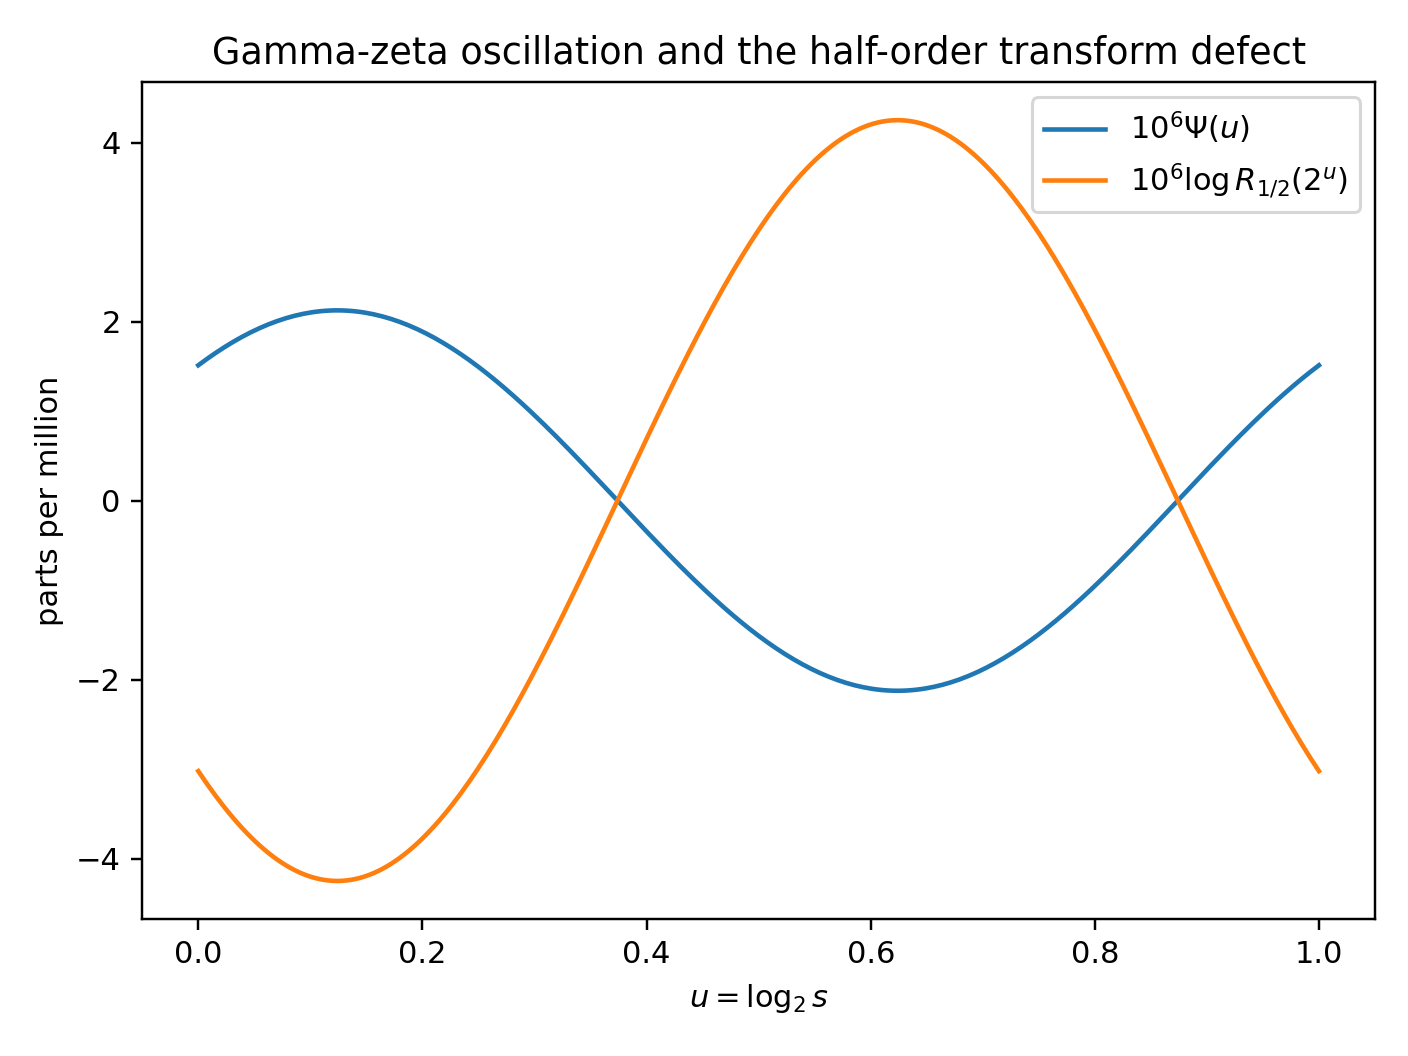
\includegraphics[width=0.86\textwidth]{gamma_zeta_fractional_defect.png}
\caption{The centered Gamma--zeta oscillation $\Psi(u)$ and the exact half-order defect
$\log R_{1/2}(2^u)=\Psi(u+1/2)-\Psi(u)$.  The vertical scale is in parts per million.}
\label{fig:gamma-zeta-defect}
\end{figure}

\begin{figure}[H]
\centering
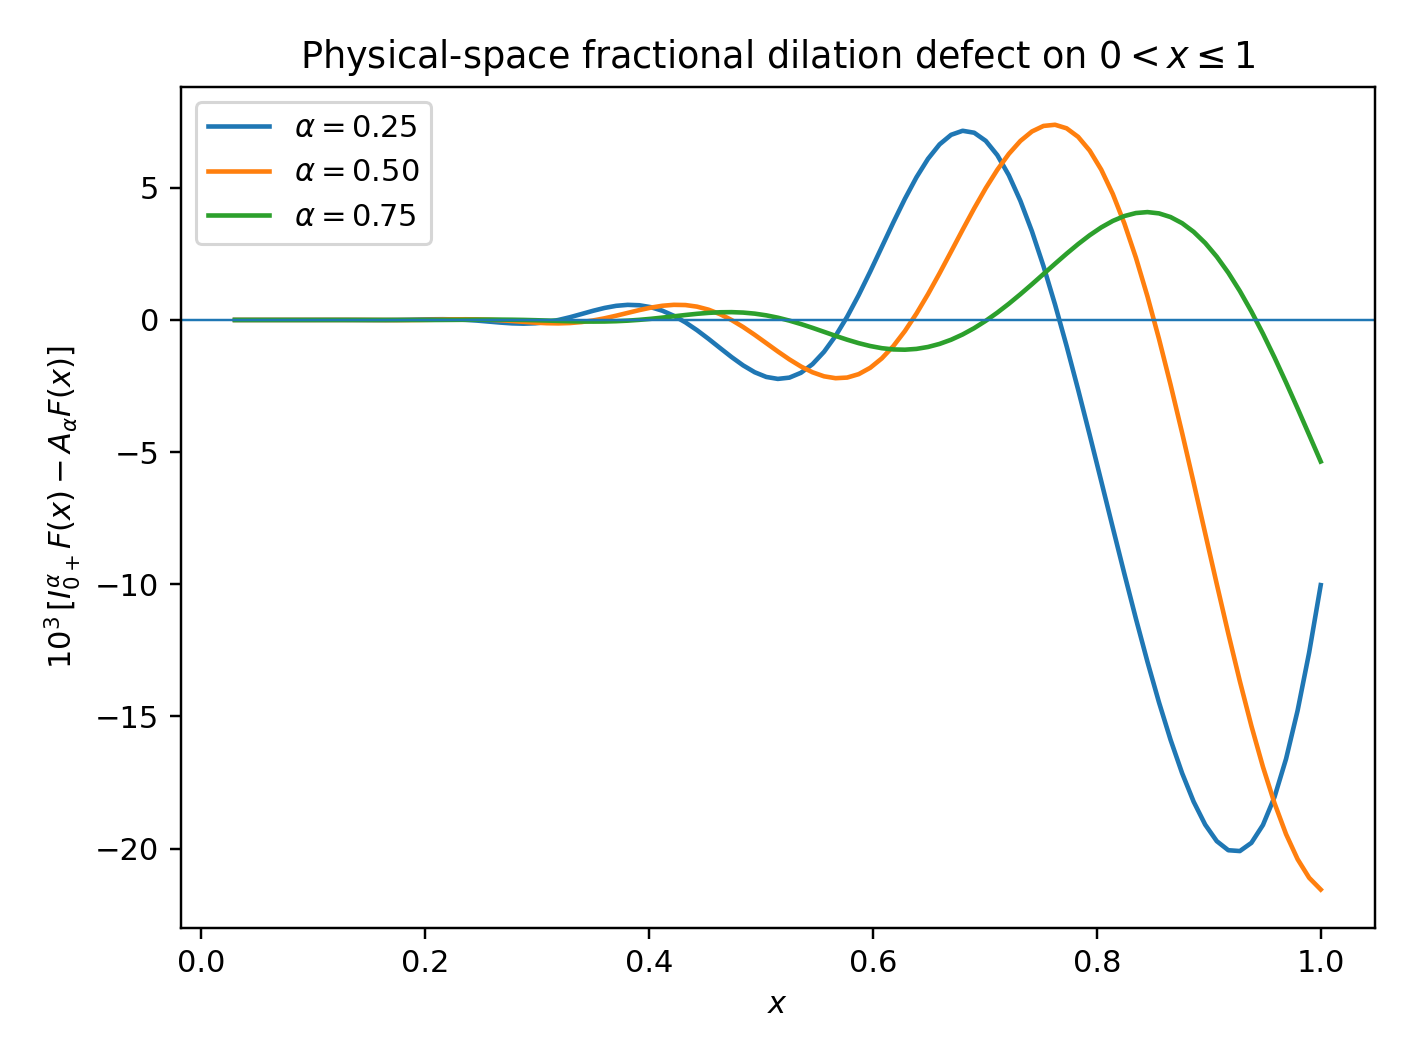
\includegraphics[width=0.86\textwidth]{fractional_dilation_defect.png}
\caption{Physical-space comparison of a Riemann--Liouville fractional integral of $F$ with
the continuous dyadic interpolation.  The visible difference is rescaled; the underlying
identity is exact only at integer order.}
\label{fig:physical-defect}
\end{figure}

\subsection{Interpretation}

The defect theorem gives a precise answer to a natural but previously ambiguous question:
what should ``half an antiderivative'' mean for the Fabius dilation equation?  There are two
canonical answers.

\begin{itemize}
\item Riemann--Liouville calculus preserves the additive order semigroup and has multiplier
$s^{-q}$.
\item Dyadic Appell interpolation preserves the exact Fabius dilation shape and the derivative
ladder $\partial_x\Aop_q=\Aop_{q-1}$.
\end{itemize}

They agree on the integer lattice.  Away from it, their ratio is not an uncontrolled error but
a smooth log-periodic multiplier with explicit Gamma--zeta Fourier coefficients.  The same
periodic object already controls the sharp Lambert-$W$ endpoint asymptotics; it therefore acts
as an obstruction simultaneously in physical endpoint asymptotics and in continuous-order
operator interpolation.

% -----------------------------------------------------------------------------
\section{Whole-line fractional operators acting on $\Up$}
\label{sec:Riesz}

The left-sided operators remember a base point.  Translation-invariant fractional calculus is
better expressed through the Riesz fractional Laplacian and potential.

\subsection{Fractional Laplacian outside the support}

For $0<\alpha<2$, use the standard singular-integral normalization
\cite{kwasnicki2017}:
\begin{equation}
 (-\Delta)^{\alpha/2}f(x)
 =C_{1,\alpha}\PV\int_{\R}\frac{f(x)-f(y)}{|x-y|^{1+\alpha}}\dd y,
 \qquad
 C_{1,\alpha}=
 \frac{2^\alpha\Gamma((1+\alpha)/2)}{\sqrt\pi\,|\Gamma(-\alpha/2)|}.
 \label{eq:fractional-Laplacian-def}
\end{equation}

\begin{theorem}[Exact exterior moment series]
\label{thm:fractional-Laplacian-tail}
For $0<\alpha<2$ and $|x|>1$,
\begin{equation}
 \boxed{
 (-\Delta)^{\alpha/2}\Up(x)
 =-C_{1,\alpha}\sum_{j=0}^{\infty}
 \frac{\poch{1+\alpha}{2j}}{(2j)!}
 \frac{m_{2j}}{|x|^{1+\alpha+2j}}.}
 \label{eq:fractional-Laplacian-tail}
\end{equation}
The series converges absolutely and locally uniformly on $|x|>1$.  This is \statusproved.
\end{theorem}

\begin{proof}
Outside the support, $\Up(x)=0$, so
\[
 (-\Delta)^{\alpha/2}\Up(x)
 =-C_{1,\alpha}\int_{-1}^{1}\frac{\Up(y)}{|x-y|^{1+\alpha}}\dd y.
\]
For $x>1$, expand
$(x-y)^{-1-\alpha}=x^{-1-\alpha}\sum_{k\ge0}\poch{1+\alpha}{k}(y/x)^k/k!$.
Odd moments vanish.  The case $x<-1$ is identical by evenness.
\end{proof}

The first terms are
\begin{equation}
 (-\Delta)^{\alpha/2}\Up(x)
 =-C_{1,\alpha}|x|^{-1-\alpha}
 \left(1+\frac{(1+\alpha)(2+\alpha)}{18x^2}
 +\frac{19(1+\alpha)_4}{16200x^4}+\cdots\right).
 \label{eq:fractional-Laplacian-first-terms}
\end{equation}
At $x=2$, six even moments reproduce direct quadrature to roughly $10^{-7}$ for the tested
orders $\alpha=0.5,0.7,1.3$; this is \statusnumeric.

\subsection{Riesz potentials}

For $0<\alpha<1$, define the one-dimensional Riesz potential with Fourier multiplier
$|t|^{-\alpha}$ by
\begin{equation}
 I_\alpha^{\mathrm R}f(x)
 =c_{1,\alpha}\int_{\R}|x-y|^{\alpha-1}f(y)\dd y,
 \qquad
 c_{1,\alpha}=
 \frac{\Gamma((1-\alpha)/2)}{2^\alpha\sqrt\pi\,\Gamma(\alpha/2)}.
 \label{eq:Riesz-potential-def}
\end{equation}

\begin{theorem}[Exterior Riesz-potential series]
\label{thm:Riesz-potential-tail}
For $0<\alpha<1$ and $|x|>1$,
\begin{equation}
 I_\alpha^{\mathrm R}\Up(x)
 =c_{1,\alpha}|x|^{\alpha-1}
 \sum_{j=0}^{\infty}
 \frac{\poch{1-\alpha}{2j}}{(2j)!}
 \frac{m_{2j}}{|x|^{2j}}.
 \label{eq:Riesz-potential-tail}
\end{equation}
The series is absolutely and locally uniformly convergent.
\end{theorem}

\begin{proof}
Expand
$|x-y|^{\alpha-1}=|x|^{\alpha-1}(1-\sgn(x)y/|x|)^{-(1-\alpha)}$ and use evenness.
\end{proof}

\subsection{Transform-side fractional derivatives}

By Fourier multiplication,
\begin{equation}
 \widehat{(-\Delta)^{\alpha/2}\Up}(t)
 =|t|^\alpha\prod_{j=1}^{\infty}\sinc(t/2^j).
 \label{eq:Riesz-transform-up}
\end{equation}
This supplies a direct integral transform for all translation-invariant fractional derivatives
of $\Up$.  It also makes the energies in \cref{eq:Sobolev-energy} the diagonal quadratic form
of the operator.

% -----------------------------------------------------------------------------
\section{The inverse Mellin transform has a Gevrey-2 boundary}
\label{sec:Gevrey}

This section uses only the audited endpoint quadratic law
\begin{equation}
 -\log F(\e^{-u})\sim\frac{u^2}{2\log2},\qquad u\to\infty.
 \label{eq:endpoint-quadratic-u}
\end{equation}
It yields a new regularity classification for the inverse Mellin transform.

Define
\begin{equation}
 A(s)=\int_0^1F(x)^s\dd x,
 \qquad \Ree s>0,
 \label{eq:A-s}
\end{equation}
and
\begin{equation}
 Q(x)=-\log F(x),
 \qquad
 a_n=\int_0^1Q(x)^n\dd x.
 \label{eq:Q-an}
\end{equation}
By \cref{eq:inverse-Mellin},
\begin{equation}
 \Mellin_G(s):=\int_0^1y^{s-1}G(y)\dd y=\frac{1-A(s)}s.
 \label{eq:MG-A}
\end{equation}

\begin{theorem}[Sharp logarithmic-moment growth]
\label{thm:an-growth}
The moments of $Q=-\log F$ satisfy
\begin{equation}
 \boxed{
 \lim_{n\to\infty}
 \left(\frac{a_n}{(2n)!}\right)^{1/n}
 =\frac1{2\log2}.}
 \label{eq:an-growth}
\end{equation}
This is \statusderived{} (using the audited endpoint quadratic law).
\end{theorem}

\begin{proof}
Put $x=\e^{-u}$.  Then
\[
 a_n=\int_0^\infty Q(\e^{-u})^n\e^{-u}\dd u.
\]
Let $c=(2\log2)^{-1}$.  For every $\varepsilon>0$, there is $U$ such that
$(c-\varepsilon)u^2\le Q(\e^{-u})\le(c+\varepsilon)u^2$ for $u\ge U$.
The upper bound splits the integral at $U$ and compares the tail with
$(c+\varepsilon)^n\Gamma(2n+1)$.  The compact part is exponentially negligible after
division by $(2n)!$.  The lower bound compares with the incomplete gamma tail
$(c-\varepsilon)^n\int_U^\infty u^{2n}\e^{-u}\dd u$, whose ratio to $(2n)!$ tends to $1$.
Take $n$th roots and then $\varepsilon\downarrow0$.
\end{proof}

\begin{theorem}[Gevrey-2 but nonanalytic inverse Mellin boundary]
\label{thm:Gevrey-barrier}
The functions $A(s)$ and $\Mellin_G(s)$ have derivatives of every order from the right at
$s=0$, with
\begin{align}
 A^{(n)}(0+)&=(-1)^na_n,\label{eq:A-derivatives-zero}\\
 \Mellin_G^{(n)}(0+)&=-\frac{A^{(n+1)}(0+)}{n+1}.
 \label{eq:MG-derivatives-zero}
\end{align}
Their formal Taylor series at $0$ have radius of convergence zero.  More precisely, the
derivative growth is of Gevrey order $2$ and of no smaller Gevrey order in the root-growth
sense.  Consequently neither transform has a holomorphic continuation through $s=0$ that
agrees with its defining integral on $\Ree s>0$.  This is \statusderived.
\end{theorem}

\begin{proof}
Every $a_n$ is finite by endpoint flatness, so differentiation under the integral from the
right gives \cref{eq:A-derivatives-zero}.  Divide the Taylor identity
$1-A(s)$ by $s$ to obtain \cref{eq:MG-derivatives-zero}.  By
\cref{eq:an-growth}, $a_n$ is asymptotic in root scale to
$c^n(2n)!$, and $(2n)!$ is of order $4^n(n!)^2$ up to subexponential factors.  Hence the
derivatives have Gevrey-2 growth.  The Taylor coefficients $a_n/n!$ have unbounded $n$th
root, so the radius is zero.  A holomorphic continuation would have a positive Taylor radius,
a contradiction.
\end{proof}

\begin{remark}
This theorem explains a sharp asymmetry.  The direct moment $\mu(s)=\E Y^s$ is entire because
it integrates against the flat density $F'$.  The inverse Mellin transform probes powers of
$F$ itself; at $s=0$ it sees the full quadratic logarithmic endpoint profile and becomes only
Gevrey-2.  The Lambert-$W$ endpoint geometry is therefore visible not only pointwise in $G$
but also as a transform-domain analyticity barrier.
\end{remark}

% -----------------------------------------------------------------------------
\section{Numerical experiments and reproducibility}
\label{sec:numerics}

The accompanying program \texttt{numerical\_experiments.py} is a verification layer, not a
source of proof.  It uses three independent representations:
\begin{enumerate}
\item exact rational cumulants and moments generated from Bernoulli numbers;
\item a finite weighted Irwin--Hall spline for
$\sum_{j=1}^{N}2^{-j}V_j$, with exact Thue--Morse inclusion--exclusion signs and the unresolved
tail replaced by its mean;
\item infinite Laplace/Fourier products and the Gamma--zeta Fourier series of $P$.
\end{enumerate}

At spline level $N=11$, the tests give:
\begin{itemize}
\item ordinary primitive errors below $2.0\times10^{-8}$ at the sampled points;
\item fractional shift errors below $1.3\times10^{-8}$;
\item fractional dyadic-lattice errors below $1.3\times10^{-8}$;
\item direct versus transmuted inverse fractional integrals agreeing to about $2.2\times10^{-10}$;
\item the mixed product value in \cref{eq:Gini-numeric};
\item exterior fractional-Laplacian moment series agreeing with direct quadrature to
      $10^{-7}$--$10^{-6}$ using six terms;
\item the exact integer-order defect $R_n=1$ and the order periodicity $R_{q+1}=R_q$ to the
      working precision.
\end{itemize}

Representative half-order values are
\begin{align}
 R_{1/2}(0.1)&=1.000004008430907\ldots,\notag\\
 R_{1/2}(1)&=0.999996976545554\ldots,\notag\\
 R_{1/2}(10)&=0.999998632323868\ldots .
 \label{eq:defect-half-numeric}
\end{align}
The complete machine-readable output is included as \texttt{numerical\_results.txt}.

\subsection{Numerical cautions}

The finite-spline formula is an alternating sum with severe cancellation if evaluated too far
on the right.  The code therefore computes only on the stable left half and imposes the exact
reflection $F(1-x)=1-F(x)$.  Fractional kernels are desingularized by substitutions before
adaptive quadrature.  The Gamma--zeta defect is evaluated at high precision because its
amplitude is only a few parts in $10^6$.

No decimal in this report is used to assert equality.  Each exact identity has an independent
symbolic proof in the preceding sections.

% -----------------------------------------------------------------------------
\section{Conjectures and research directions}
\label{sec:future}

\subsection{Higher inverse derivatives}

The first inverse derivative has the sharp threshold in \cref{thm:inverse-slope-Lr}.  The
Lambert endpoint heuristic suggests a complete hierarchy.

\begin{conjecture}[Higher inverse-derivative threshold]
\label{conj:higher-G-derivatives}
For every integer $n\ge1$ and $r>0$,
\begin{equation}
 G^{(n)}\in L^r(0,1)
 \quad\Longleftrightarrow\quad
 0<r\le\frac1n.
 \label{eq:conj-higher-G}
\end{equation}
\statusopen
\end{conjecture}

A formal endpoint differentiation of
$G(y)\approx\exp[-\sqrt{2\log2\,\log(1/y)}]$ predicts
$G^{(n)}(y)\approx y^{-n}G(y)$ times powers of $\log(1/y)$.  After $y=\e^{-v}$, the $L^r$
integrand has leading exponential $\exp((nr-1)v-r\sqrt{2Lv})$, giving exactly the stated
threshold, including convergence on the boundary $nr=1$.

\subsection{Fractional endpoint transseries}

\begin{conjecture}[Shifted Lambert--Gamma--zeta transseries]
\label{conj:fractional-transseries}
For fixed noninteger $\alpha$, the functions
$I_{0+}^{\alpha}F(x)$ and $D_{0+}^{\alpha}F(x)$ admit full small-$x$ transseries in the same
lower-Lambert coordinate as $F$, with the periodic Gamma--zeta phase shifted explicitly by
$\alpha$.  The leading logarithmic quadratic term is unchanged; the algebraic prefactor and
periodic phase acquire computable $\alpha$-dependent corrections.
\statusopen
\end{conjecture}

The Bromwich representations \cref{eq:Bromwich-J,eq:Bromwich-D} make this a concrete saddle
problem.  Multiplication by $s^{\mp\alpha}$ changes the logarithmic saddle equation by an
additive $\alpha\log s$, while the periodic $P(\log_2s)$ survives.

\subsection{Physical-space sign structure of the dyadic defect}

Define for $q>0$
\begin{equation}
 \Delta_q(x)=I_{0+}^{q}\extF(x)-\Aop_q\extF(x).
 \label{eq:physical-defect}
\end{equation}
Its Laplace transform is known exactly from \cref{thm:fractional-defect}, but its zeros and
sign changes in physical space are not.

\begin{conjecture}[Finite sign complexity on a dyadic cell]
For every $q\in(0,1)$, $\Delta_q$ has finitely many sign changes on $[0,1]$, and their number
is uniformly bounded in $q$.  The symmetry $q\leftrightarrow1-q$ visible in the dominant
Fourier mode of the multiplier should induce an approximate pairing of zero locations.
\statusopen
\end{conjecture}

A rigorous attack could combine complete monotonicity of Laplace kernels, variation-diminishing
estimates, and a certified interval evaluation of the Gamma--zeta series.

\subsection{A Jackson or $q$-fractional calculus at base $1/2$}

The repository's Gaussian-binomial and half-base $q$-Pochhammer formulas suggest that the
dyadic Appell family may be only one coordinate of a richer $q=1/2$ fractional calculus.
Promising goals are:
\begin{itemize}
\item construct a Jackson-type fractional integral whose integer values reproduce the exact
      repeated Fabius primitives;
\item identify its semigroup defect as a $q$-cocycle related to \cref{eq:Appell-cocycle};
\item express its values at dyadic rationals by analytic continuations of Gaussian-binomial
      coefficients;
\item compare its Mellin symbol with the Gamma--zeta multiplier $R_q$.
\end{itemize}
This direction may provide the most direct bridge from fractional calculus to the repository's
$q$-binomial arithmetic.

\subsection{Arithmetic and closed forms for Sobolev energies}

The energies $\mathcal E_{2m}=\|\Up^{(m)}\|_2^2$ and their fractional analogues are natural
periods of the infinite sinc product.  It is unknown whether any nontrivial member has a
closed form in familiar constants.

\begin{conjecture}[No elementary gamma--zeta reduction for generic energy]
Except for identities forced by scaling or Parseval, the values $\mathcal E_\alpha$ at generic
rational $\alpha\ge0$ are not finite combinations of algebraic numbers, powers of $\pi$, and
ordinary zeta values.  They should instead define a new family of dyadic sinc periods.
\statusopen
\end{conjecture}

Useful next steps are high-precision computation, integer-relation searches with strict
complexity penalties, Mellin--Barnes representations, and comparison with the spectral zeta
already developed for the zero divisor of $\Phiup$.

\subsection{Nonlinear fractional Volterra equations for $G$}

Equation \cref{eq:inverse-RL} can be read as a nonlinear Volterra equation because $G$ occurs
both as the integration limit and as the inverse hidden in $F$.  Differentiating in $y$ gives a
family of Abel-type equations.  Questions include uniqueness in weighted Holder classes,
stable numerical inversion, and whether the order variable $\alpha$ can be used as a
regularization parameter for computing $G$ near its singular endpoints.

\subsection{Complex order and monodromy}

The operator $\Aop_q$ is entire in complex $q$ after a branch for $2^q$ is fixed.  The exact
defect becomes
\[
 R_q(s)=\exp(P(\log_2s+q)-P(\log_2s)).
\]
For complex $q$, the Fourier series of $P$ grows in one imaginary direction and decays in the
other.  Determining the maximal strip of analytic continuation, the zero/pole structure of
$R_q$, and the monodromy of complex-order fractional inversions is a concrete frontier
problem.

\subsection{Formalization program}

A practical Lean development can proceed in increasing order of analytic difficulty:
\begin{enumerate}
\item prove the integer primitive ladder and weighted polynomial formulas from the existing
      global dilation API;
\item add a minimal Riemann--Liouville kernel API and prove the order-shift identity;
\item formalize the moment endpoint and fractional dyadic lattice;
\item formalize monotone substitutions for $F$ and $G$, yielding the inverse transmutation
      theorem;
\item define $\Aop_q$ and prove the cocycle and derivative ladder;
\item combine the existing exact periodic decomposition with the Thue--Morse Laplace product
      to formalize the defect and rigidity theorem;
\item only then address Riesz kernels and the Gevrey boundary theorem.
\end{enumerate}
The first five stages require mostly real integration, Gamma identities, and existing Fabius
lemmas.  The sixth stage reuses the strongest current Gamma--zeta formalization and would make
the report's flagship theorem machine checked.

% -----------------------------------------------------------------------------
\section{Summary of exact formulas}
\label{sec:summary-formulas}

For convenience, the principal identities are collected here.

\begin{longtable}{@{}p{0.30\textwidth}p{0.64\textwidth}@{}}
\toprule
Object & Exact formula \\
\midrule
\endhead
First primitive & $\displaystyle \int_0^xF(t)\dd t=F(x/2)$, $0\le x\le1$.\\[0.4em]
$n$th primitive & $\displaystyle I_{0+}^nF(x)=2^{\binom n2}F(x/2^n)$.\\[0.4em]
$n$th derivative & $\displaystyle \extF^{(n)}(x)=2^{\binom{n+1}{2}}\extF(2^nx)$.\\[0.4em]
Up CDF & $\displaystyle \int_{-\infty}^x\Up(t)\dd t=F((x+1)/2)$.\\[0.4em]
Weighted fractional primitive & $\displaystyle I^\alpha[t^pF]=\sum_{k=0}^p(-1)^k\binom pk(\alpha)_kx^{p-k}\J_{\alpha+k}$.\\[0.4em]
Inverse primitive & $\displaystyle \int G(y)\dd y=yG(y)-F(G(y)/2)+C$.\\[0.4em]
Inverse fractional integral & $\displaystyle I^\alpha G(y)=\Gamma(\alpha+1)^{-1}\int_0^{G(y)}(y-F(x))^\alpha\dd x$.\\[0.4em]
Inverse fractional derivative & $\displaystyle D^\alpha G(y)=\Gamma(1-\alpha)^{-1}\int_0^{G(y)}(y-F(x))^{-\alpha}\dd x$, $0<\alpha<1$.\\[0.4em]
Mellin transform & $\displaystyle \int_0^1x^{s-1}F(x)\dd x=(1-\mu(s))/s$.\\[0.4em]
Fractional endpoint & $\displaystyle \J_\alpha(1)=\mu(\alpha)/\Gamma(\alpha+1)$.\\[0.4em]
Fractional dyadic lattice & $\displaystyle \J_\beta(2^{-n})=2^{-n\beta-\binom n2}\mu(n+\beta)/\Gamma(n+\beta+1)$.\\[0.4em]
Laplace transform & $\displaystyle \Laplace F(s)=\phi(s)/s$.\\[0.4em]
Fourier transform of $\Up$ & $\displaystyle \widehat\Up(t)=\prod_{j\ge1}\sinc(t/2^j)$.\\[0.4em]
Dyadic Appell family & $\displaystyle \Aop_q\extF(x)=2^{q(q-1)/2}\extF(2^{-q}x)$.\\[0.4em]
Exact fractional defect & $\displaystyle R_q(s)=\exp(P(\log_2s+q)-P(\log_2s))$.\\[0.4em]
Riesz tail & $\displaystyle (-\Delta)^{\alpha/2}\Up(x)=-C_{1,\alpha}\sum_{j\ge0}(1+\alpha)_{2j}m_{2j}/((2j)!|x|^{1+\alpha+2j})$.\\[0.4em]
Inverse Mellin boundary & $\displaystyle \lim_{n\to\infty}(a_n/(2n)!)^{1/n}=1/(2\log2)$.\\
\bottomrule
\end{longtable}

% -----------------------------------------------------------------------------
\appendix
\section{Detailed proof supplements}
\label{app:proofs}

\subsection{Entire continuation in power exponents}

A recurring statement above is that an apparently restricted Mellin integral is entire.  The
mechanism is endpoint flatness.  If $h\in C^\infty([0,1])$ and every derivative of $h$ vanishes
at $0$, then for each $N$ there is $C_N$ with $|h(x)|\le C_Nx^N$ on $[0,1]$.  Hence
\[
 \int_0^1x^sh(x)\dd x
\]
converges locally uniformly for $\Ree s>-N-1$.  Since $N$ is arbitrary, the Mellin transform
is entire.  This applies to $F$, $F'$, and every $F^{(n)}$ near the left endpoint.  It also
justifies differentiation under the integral and the analytic continuation used in
\cref{eq:F-derivative-moments,eq:dyadic-shell}.

\subsection{Moment recurrence}

The distributional fixed point
\begin{equation}
 Y\overset d=\frac{V+Y'}2,
 \label{eq:Y-fixed-point}
\end{equation}
with $V\sim\mathrm{Unif}[0,1]$ and $Y'\overset d=Y$ independent gives, for integer $n\ge1$,
\begin{equation}
 (2^n-1)\mu_n
 =\sum_{k=0}^{n-1}\binom nk\frac{\mu_k}{n-k+1}.
 \label{eq:moment-recurrence}
\end{equation}
This is a convenient exact alternative to the Bell-polynomial construction.  The two methods
provide independent symbolic checks of the moment table.

\subsection{Why the inverse Mellin integral stops at $\Ree s=0$}

For $\Ree s<0$, $F(x)^s=\exp(|\Ree s|Q(x))$.  With $x=\e^{-u}$ and
$Q(\e^{-u})\sim cu^2$, the integrand behaves like
$\exp(|\Ree s|cu^2-u)$, which is not integrable.  Thus $A(s)$ has a genuine natural boundary
for its defining integral at $\Ree s=0$.  The transform $\Mellin_G(s)$ itself remains finite at
$s=0$, but its derivatives exhibit the same Gevrey-2 growth and it cannot cross the boundary
analytically.

\subsection{A compact derivation of the Gamma--zeta defect}

Writing $u=\log s$, $v=u/L$, \cref{eq:exact-signed-log} is
\[
 \log\mathscr L(s)=-\frac{u^2}{2L}-\frac u2+P(v).
\]
The transform of $\Aop_q\extF$ is
$2^{q(q+1)/2}\mathscr L(2^qs)$.  Therefore
\begin{align*}
 \log R_q(s)
 &=\frac{q(q+1)}2L+qu
   +\log\mathscr L(\e^{u+qL})-\log\mathscr L(\e^u)\\
 &=P(v+q)-P(v).
\end{align*}
Every polynomial term cancels.  This cancellation is why the tiny periodic correction is not a
secondary asymptotic detail here: it is the entire noninteger defect.

\section{Numerical files and execution}
\label{app:numerical-files}

The archive contains:
\begin{itemize}
\item \texttt{numerical\_experiments.py}: the fully commented Python program;
\item \texttt{numerical\_results.txt}: exact moments and numerical checks;
\item \texttt{moment\_table.tex}: the generated rational moment table;
\item \texttt{fractional\_dilation\_defect.png}: physical-space comparison;
\item \texttt{gamma\_zeta\_fractional\_defect.png}: transform multiplier plot.
\end{itemize}

Run from the report directory with
\begin{lstlisting}[language=bash]
python numerical_experiments.py
\end{lstlisting}
The program requires Python 3 with \texttt{numpy}, \texttt{scipy}, \texttt{sympy},
\texttt{mpmath}, and \texttt{matplotlib}.  All output paths are relative to the script.

\section{Audit notes and source map}
\label{app:audit-map}

The recursive audit was organized by mathematical lineage rather than by filename count.
The principal living inputs were:
\begin{itemize}
\item the formal-primary exposition \texttt{Fabius\_Function\_and\_Rvachev\_Up.tex};
\item the consolidated \texttt{non-formalized-research-frontiers.tex};
\item the mathematical glossary and Lean walkthrough;
\item active drafts on arithmetic/dyadic sampling, inverse asymptotics, Newton--Rvachev
      hierarchies, half-integer spectral identities, and sinc-product Fourier decay;
\item corrected/transcribed primary papers by Fabius, Rvachev, and Arias de Reyna as retained
      in the repository.
\end{itemize}

Searches for exact or near-exact counterparts of the new formulas used both terminology and
formula fragments.  In particular, no current-lineage match was found for the
Riemann--Liouville order shift \cref{eq:fractional-shift}, the quantile transmutation
\cref{eq:F-to-G-transmutation,eq:G-to-F-transmutation}, the exact defect
\cref{eq:defect-exact}, or the Gevrey limit \cref{eq:an-growth}.  The audit does not exclude an
independent result elsewhere in the mathematical literature.

% -----------------------------------------------------------------------------
\begin{thebibliography}{99}

\bibitem{fabius1966}
J. Fabius,
\newblock A probabilistic example of a nowhere analytic $C^\infty$-function,
\newblock \emph{Zeitschrift fuer Wahrscheinlichkeitstheorie und Verwandte Gebiete}
\textbf{5} (1966), 173--174.

\bibitem{rvachev1971}
V. L. Rvachev,
\newblock On a finite function,
\newblock \emph{Doklady Akademii Nauk Ukrainian SSR}, Series A (1971), no. 8, 705--707.

\bibitem{rvachev1990}
V. L. Rvachev,
\newblock Compactly supported solutions of functional-differential equations and their
applications,
\newblock \emph{Russian Mathematical Surveys} \textbf{45} (1990), no. 1, 87--120.

\bibitem{arias1982}
J. Arias de Reyna,
\newblock On the Fabius function,
\newblock original Spanish article (1982); English translation and source copy retained in the
project documentation.

\bibitem{arias2018}
J. Arias de Reyna,
\newblock Arithmetic of the Fabius function,
\newblock \emph{INTEGERS} \textbf{18} (2018), Paper A48; arXiv:1702.06487.

\bibitem{allouche2003}
J.-P. Allouche and J. Shallit,
\newblock \emph{Automatic Sequences: Theory, Applications, Generalizations},
\newblock Cambridge University Press, 2003.

\bibitem{samko}
S. G. Samko, A. A. Kilbas, and O. I. Marichev,
\newblock \emph{Fractional Integrals and Derivatives: Theory and Applications},
\newblock Gordon and Breach, 1993.

\bibitem{caputo1967}
M. Caputo,
\newblock Linear models of dissipation whose $Q$ is almost frequency independent--II,
\newblock \emph{Geophysical Journal of the Royal Astronomical Society} \textbf{13} (1967),
529--539.

\bibitem{kwasnicki2017}
M. Kwasnicki,
\newblock Ten equivalent definitions of the fractional Laplace operator,
\newblock \emph{Fractional Calculus and Applied Analysis} \textbf{20} (2017), 7--51;
arXiv:1507.07356.

\bibitem{cong2021}
N. D. Cong,
\newblock Semigroup property of fractional differential operators and its applications,
\newblock arXiv:2107.08914, 2021.

\bibitem{corless1996}
R. M. Corless, G. H. Gonnet, D. E. G. Hare, D. J. Jeffrey, and D. E. Knuth,
\newblock On the Lambert $W$ function,
\newblock \emph{Advances in Computational Mathematics} \textbf{5} (1996), 329--359.

\bibitem{project-primary}
V. Reshetnikov et al.,
\newblock \emph{The Fabius Function and Rvachev Up: definitions, equivalences, arithmetic,
asymptotics, and formalization map},
\newblock living LaTeX exposition in the \texttt{ProveIt} repository, accessed 27 August 2026.

\bibitem{project-frontier}
V. Reshetnikov et al.,
\newblock \emph{Non-formalized research frontiers for the Fabius and Rvachev functions},
\newblock consolidated LaTeX frontier volume in the \texttt{ProveIt} repository, accessed
27 August 2026.

\end{thebibliography}

\end{document}
